\chapter{计算CTL下的遗忘:基于归结的方法}\label{chapter04}
{\em 
已有结果显示,任意的$\CTL$公式可以转换为$\CTLsnf$子句的集合。归结是一种以子句为计算对象的判断可满足性的方法,本章提出一种基于归结的计算遗忘理论的方法。
其主要思想是:首先将给定的$\CTL$公式转换为$\CTLsnf$子句的集合,其次在相应的原子命题上使用归结规则得到归结结果,最后“消除”之前引入的索引和$\start$,最终得到遗忘的结果。其主要流程图如图~\ref{Fig:chapter05:v1uv2}所示。
正如本章所要说明的那样,$\CTL$不具有均匀插值这一属性,基于归结的方法在有的情况下是不能计算出遗忘结果的。然而,在有些$\CTL$子类下,本章提出的方法能够计算出其遗忘结果。}
\begin{figure*}[!htb]
	\centering
	% Requires \usepackage{graphicx}
	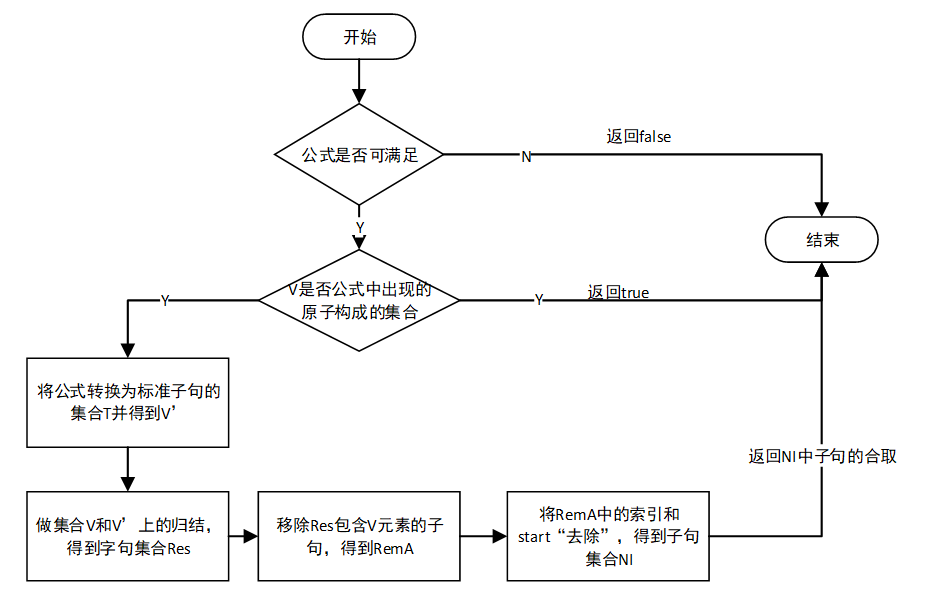
\includegraphics[width=15cm]{chapter04/frame.png}\\
	\caption{基于归结的遗忘的主要流程图}
	\label{Fig:chapter05:v1uv2}
\end{figure*}

\section{引言}
本章展示如何使用表~\ref{tab:res}中的归结规则来计算$\CTL$下的遗忘理论。
在本章给定如下约定的记号。令$V\subseteq \Ha$是要遗忘的原子命题的集合,$I\subseteq \Ind$是索引的集合,$V'$表示计算过程所引入的原子命题的集合且满足$V'\cap V=\emptyset$。
此外,$\varphi$是$\CTL$公式,且$T_{\varphi}$是在$\varphi$上使用表~\ref{tab:trans}中的转换规则得到的$\CTLsnf$子句的集合。
显然可以知道,$V'=\Var(T_{\varphi})-\Var(\varphi)$。
在不另加说明的情况下$\Hm$表示五元组$(S,R,L,[\_],s_0)$。
此时,本章所设计的算法的伪代码如算法~\ref{alg:compute:forgetting:by:Resolution}所示。

\begin{algorithm}[htbp]
	\small
	\setstretch{1.2}
	\caption{\emph{ERes}$(\varphi, V)$}
	\label{alg:compute:forgetting:by:Resolution}
	\begin{algorithmic}[1]
		\REQUIRE ~~\\
		\begin{tabular}[t]{p{8mm}l}
			$\varphi$&:$\CTL$公式\\
			$V$&:需要遗忘的原子命题的集合
		\end{tabular}
		\ENSURE ~~\\
		\begin{tabular}[t]{p{8mm}l}
			$ERes(\varphi, V)$&\qquad:公式的合取
			%$SD$&:鞍点策略的支付量
		\end{tabular}
		\IF{$\varphi$ 是不可满足的}
		\RETURN $\bot$;
		\ENDIF
		\IF{$V=\Var(\varphi)$}
		\RETURN $\bot$;
		\ENDIF
		\STATE $T_{\varphi}, V', I \lto \emph{Transform}(\varphi)$;
		\STATE $Res \lto \emph{Resolution}(T_{\varphi}, V\cup V')$;
		\STATE $\emph{RemA} \lto \emph{Removing\_atoms}(Res, V)$;
		\STATE $\NI \lto \emph{Removing\_index}(\emph{RemA})$;
		\RETURN $\bigwedge_{\psi \in \NI_{\CTL}} \psi$;
	\end{algorithmic}
\end{algorithm}


算法~\ref{alg:compute:forgetting:by:Resolution}对于输入$\varphi$和$V$,输出结果记为$ERes(\varphi, V)$。
为了实现这一目标,需要解决如下两个主要问题:
\begin{itemize}
	\item[(1)] 如何表示$\CTL$公式和带索引的$\CTL$公式之间的关系?如在第三章中所展示的那样,将一个$\CTL$公式转换为$\CTLsnf$子句的集合会引入新的原子命题和索引。虽然已有的研究说明了$\CTL$公式可以转换为带索引的公式的集合并保证其可满足性,然而并没有表明这两种形式的公式之间的模型具有怎样的联系。本章给出一种扩展的互模拟定义,以描述两种公式的模型之间的关系。
	\item[(2)] 如何“移除”无关的原子命题(包括需要遗忘的原子命题和转换过程中引入的新的原子命题),以及如何“消除”索引?为此,本章给出“移除”原子命题的一般操作,对应算法~\ref{alg:compute:forgetting:by:Resolution}中的$\emph{Removing\_atoms}(Res, V)$过程,并提出一种一般化的Ackermann引理。为了“消除”索引,探索几个几个逻辑等价关系,对应算法~\ref{alg:compute:forgetting:by:Resolution}中的$\emph{Removing\_index}(\emph{RemA})$过程。
\end{itemize}

本章其余部分组织如下:首先,第\ref{chapter4:sub:biVB}节给出二元互模拟的定义及其相关性质。其次,第\ref{chapter4:transform}节介绍将$\CTL$公式转换为$\CTLsnf$子句的集合的过程。第\ref{chapter4:resolution}节阐述基于归结的计算过程。

第\ref{chapter05-optimal-model}节阐述本章针对权衡隐私与效用问题所提出的优化模型,并形式化的给出模型表述。第\ref{chapter05-optimazation-mechanism} 节对本章提出优化模型的求解方法及算法进行详细的阐述。第\ref{chapter04-experiment}节利用公开数据集对所提出的方法和算法进行实验分析。最后,第\ref{chapter04-conclusion}节对本章的主要工作进行总结。

\section{二元互模拟}
\label{chapter4:sub:biVB}
对于给定的初始$\Ind$-结构,这里定义一种$\tuple{V, I}$-互模拟关系。为了与一元的(只考虑原子命题的集合)$V$-互模拟对应,称$\tuple{V, I}$-互模拟为二元互模拟。其在$V$-互模拟的基础上又考虑了索引的集合在结构间关系。
\begin{definition}[二元互模拟] \label{def:VInd:bisimulation}
	令$V\subseteq \Ha$、$I\subseteq \Ind$分别是原子命题和索引的集合,$\Hm_i=(S_i, R_i, L_i, [\_],s_0^i)$ $(i=1,2)$是$\Ind$-Kripke结构,${\cal K}_i=(\Hm_i,s^i)$是初始$\Ind$-结构。称${\cal K}_1$和${\cal K}_2$是$\tuple{V, I}$-互模拟的(记为${\cal K}_1 \lrto_{\tuple{V, I}} {\cal K}_2$),当且仅当${\cal K}_1 \lrto_V {\cal K}_2$且$\forall j\in (\Ind - I)$有:
	\begin{itemize}
		\item 对任意的$(s,s_1) \in [j]_1$,存在$(s',s_1')\in [j]_2$使得$s\lrto_V s'$且$s_1 \lrto_V s_1'$;
		\item 对任意的$(s',s_1') \in [j]_2$,存在$(s,s_1)\in [j]_1$使得$s\lrto_V s'$且$s_1 \lrto_V s_1'$。
	\end{itemize}
	
\end{definition}

由定义~\ref{def:VInd:bisimulation}可知,当探讨的公式为$\CTL$公式时,因为不用考虑索引,$\lrto_{\tuple{V, I}}$“降维”为$\lrto_V$。
与$\lrto_V$类似,$\lrto_{\tuple{V, I}}$在本文中至关重要的两个性质如下。
\begin{proposition}\label{pro:VI:div}
	令$V_1,V_2\subseteq \Ha$为原子命题的集合,$I_1, I_2 \subseteq \Ind$为索引的集合,${\cal K}_i = (\Hm_i, s_0^i)$ $(i=1,2,3)$为初始$\Ind$-结构。若${\cal K}_1 \lrto_{\tuple{V_1,I_1}} {\cal K}_2$、${\cal K}_2 \lrto_{\tuple{V_2,I_2}} {\cal K}_3$,则:
	\begin{itemize}
		\item[(i)] ${\cal K}_1 \lrto_{\tuple{V_1\cup V_2,I_1\cup I_2}} {\cal K}_3$;
		\item[(ii)] 如果$V_1 \subseteq V_2$且$I_1 \subseteq I_2$,则${\cal K}_1 \lrto_{\tuple{V_2,I_2}} {\cal K}_2$。
	\end{itemize}
\end{proposition}
\begin{proof}
	(i) 由定义~\ref{def:VInd:bisimulation}可知${\cal K}_1 \lrto_{V_1} {\cal K}_2$、${\cal K}_2 \lrto_{V_2} {\cal K}_3$,因此由命题~\ref{pro:div}可知${\cal K}_1 \lrto_{V_1\cup V_2} {\cal K}_3$。
	
	${\cal K}_1 \lrto_{\tuple{V_1,I_1}} {\cal K}_2$\\
	$\Rto$ $\forall j\in (\Ind-(I_1\cup I_2))$有:$\forall(s,s_1) \in [j]_1$,$\exists (s', s_1')\in [j]_2$使得$s\lrto_{V_1} s'$,$s_1\lrto_{V_1} s_1'$\\
	$\Rto$ 又因为${\cal K}_2 \lrto_{\tuple{V_2,I_2}} {\cal K}_3$,所以$\exists (s'', s_1'')\in [j]_3$使得$s'\lrto_{V_2} s''$,$s_1'\lrto_{V_2} s_1''$  \hfill \\
	$\Rto$ $s \lrto_{V_1\cup V_2} s''$且$s_1 \lrto_{V_1\cup V_2} s_1''$
	
	同理可证,$\forall (s'',s_1'')\in [j]_3$,$\exists (s,s_1)\in [j]_1$使得$s \lrto_{V_1\cup V_2} s''$且$s_1 \lrto_{V_1\cup V_2} s_1''$。
	因此,由定义~\ref{def:VInd:bisimulation}可知${\cal K}_1 \lrto_{\tuple{V_1\cup V_2,I_1\cup I_2}} {\cal K}_3$。
	
	(ii)可以由命题~\ref{pro:div}中的(ii)可得。
\end{proof}

对于给定的$\Ind$-Kripke结构$\Hm=(S,R,L,[\_],s_0)$和$\Hm'=(S',R',L',[\_],s_0')$,$\Hm$和$\Hm'$之间的二元互模拟关系$\lrto_{\tuple{V,I}}$给描述公式间在二元组$\tuple{V,I}$上的等价关系提供了前提条件。这同时也为解决本章引言部分提出的问题$(1)$奠定了基础。

\begin{definition}
	给定两个公式(或公式的集合)$T_1$和$T_2$,$I\subseteq \Ind$是索引的集合,$V''\subseteq \Ha$是原子命题的集合。如果下面条件被满足,则称$T_1$和$T_2$在二元组$\tuple{V,I}$上逻辑等价(记为$T_1\equiv_{\tuple{V,I}} T_2$):
	\begin{itemize}
		\item $\forall (\Hm,s_0)\in \Mod(T_1)$,$\exists (\Hm',s_0')\in \Mod(T_2)$使得$(\Hm,s_0) \lrto_{\tuple{V, I}} (\Hm',s_0')$,且
		\item $\forall (\Hm',s_0')\in \Mod(T_2)$,$\exists (\Hm,s_0)\in \Mod(T_1)$使得$(\Hm,s_0) \lrto_{\tuple{V, I}} (\Hm',s_0')$。
	\end{itemize}
	
\end{definition}

在后面的小节中,将围绕之前提出的两个问题和算法~\ref{alg:compute:forgetting:by:Resolution}中的几个关键步骤(第7到第11行)来证明$ERes(\varphi, V) \equiv_{\tuple{V',\emptyset}} \CTLforget(\varphi, V)$。在这个等价关系中$\varphi$为$\CTL$公式,$V$为需要遗忘的原子命题的集合,$V'$是将$\varphi$转换为$\CTLsnf$子句集合过程中引入的新的原子命题的集合。这个结论告诉我们,如果$ERes(\varphi, V)$公式中不包含$V'$的元素,或者$\IR(ERes(\varphi, V), V')$,则$ERes(\varphi, V)$就是从$\varphi$中遗忘掉$V$中的原子命题之后得到的结果。

\section{将$\CTL$公式转换为$\CTLsnf$子句的集合}
将$\CTL$公式$\varphi$转换为$\CTLsnf$子句的集合这一过程(记为$Trangsform(\varphi)$)对应算法~\ref{alg:compute:forgetting:by:Resolution}中的第7行所代表的过程。
对于输入$\varphi$,该过程事先将$\varphi$转换为其否定范式(记为$\nnf(\varphi)$),然后通过下面的等价关系\cite{zhang2014resolution,DBLP:books/el/leeuwen90/Emerson90}将出现在公式中的$\top$和$\bot$“去掉”(记为$\simp(\nnf(\varphi))$)。
\begin{align*}
	& (\varphi \wedge \top) \equiv \varphi && (\varphi \wedge \bot) \equiv \bot && (\varphi \vee \top)\equiv \top && (\varphi \vee \bot) \equiv \varphi \\
	& \neg \top \equiv \bot && \neg \bot \equiv \top && QT \bot \equiv \bot && QT \top \equiv \top  \\
	& Q(\varphi \UNTILL \bot) \equiv \bot  && Q(\varphi \UNTILL \top) \equiv \top && Q(\bot \UNTILL \varphi) \equiv \varphi && Q(\top \UNTILL \varphi) \equiv Q\FUTURE \varphi\\
	& Q(\varphi \UNLESS \bot) \equiv Q \GLOBAL \varphi  && Q(\varphi \UNLESS \top) \equiv \top && Q(\bot \UNLESS \varphi) \equiv \varphi && Q(\top \UNLESS \varphi) \equiv \top
\end{align*}
在上述等价关系中,$Q\in \{\ALL,\EXIST\}$是路径量词,$T\in \{\FUTURE, \GLOBAL, \NEXT\}$是时序操作符。

在得到$\simp(\nnf(\varphi))$后,将$T_{\varphi}$初始化为$\{\ALL \GLOBAL(\start \rto p), \ALL \GLOBAL(p \rto \simp(\nnf(\varphi)))\}$,然后转换过程从表~\ref{tab:trans}中找到匹配的规则来将$T_{\varphi}$中的非$\CTLsnf$子句形式的公式转换为$\CTLsnf$子句,并将得到的结果更新$T_{\varphi}$直到$T_{\varphi}$中不存在非$\CTLsnf$子句形式的公式。这个转换过程被写为算法~\ref{alg:compute:trans}。


\begin{algorithm}[htbp]
	\small
	\setstretch{1.2}
	\caption{\emph{Transform}$(\varphi)$}
	\label{alg:compute:trans}
	\begin{algorithmic}[1]
		\REQUIRE ~~\\
		\begin{tabular}[t]{p{8mm}l}
			$\varphi$&:$\CTL$公式
		\end{tabular}
		\ENSURE ~~\\
		\begin{tabular}[t]{p{8mm}l}
			$T_{\varphi}$&: $\CTLsnf$子句的集合\\
			$V'$& : 新引入的原子命题的集合\\
			$I$ &: 引入的索引的集合
			%$SD$&:鞍点策略的支付量
		\end{tabular}
		\STATE $T_{\varphi}\lto \{\ALL \GLOBAL(\start \rto p), \ALL \GLOBAL(p \rto \simp(\nnf(\varphi)))\}$;(其中$p\in {\cal A}-var(\varphi)$)
		\STATE $V'\lto \{p\}$;
		\STATE $I\lto \emptyset$;
		\WHILE{$\exists \psi \in T_{\varphi}$使得$\psi$不是$\CTLsnf$子句}
		\STATE $T_{\varphi} \lto T_{\varphi}-\{\psi\}$;
		\STATE $T_{\varphi} \lto Trans(\psi) \cup T_{\varphi}$;
		\IF{$Trans(\psi)$引入了一个新原子命题$q$}
		\STATE $V'\lto V' \cup \{q\}$;
		\ENDIF
		\IF{$Trans(\psi)$引入了一个新的索引$ind$}
		\STATE $I\lto I \cup \{ind\}$;
		\ENDIF
		\ENDWHILE
		\RETURN $T_{\varphi}, V', I$;
	\end{algorithmic}
\end{algorithm}


在算法~\ref{alg:compute:trans}中,$Trans(\psi)$表示使用表~\ref{tab:trans}中的某一条规则来转换$\psi$(规则中长横线上面的部分),并返回规则的结果(规则中长横线下面的部分)、引入的新原子命题和索引。这里使用规则\textbf{Trans(6)}为例来描述这一过程。令$\psi=q \rto \ALL \NEXT \phi$,可以看出当$\phi$不是经典子句的时候$\psi$不是$\CTLsnf$子句,且规则\textbf{Trans(6)}是能使用的(匹配的)规则,则$Trans(\psi)$对$\psi$使用规则\textbf{Trans(6)}并返回结果$\{q \rto \ALL \NEXT q', q' \rto \phi\}$(在这里,引入了新的原子命题$q'$,但是没有引入新的索引)。

\begin{proposition}\label{pro:TranE}
	令$\varphi$是一个$\CTL$公式,$(T_{\varphi}, V', I) = Transform(\varphi)$,则$\varphi \equiv_{\tuple{V',I}} T_{\varphi}$。
\end{proposition}
\begin{proof}
	为了讨论方便,令$Transform(\varphi)$过程产生了一个公式集合的序列,$T_0, T_1, \dots, T_n=T_{\varphi}$,其中$p$是不出现在$\varphi$中的原子命题,$T_0=\{\ALL \GLOBAL(\start \rto p), \ALL \GLOBAL(p \rto \simp(\nnf(\varphi)))\}$且对任意的$i$($0\leq i < n$)有$T_{i+1} = (T_i-\{\psi\}) \cup R_i$($Trans(\psi)$返回的结果为$R_i$)。此外,在这一过程中,所有的公式都是其否定范式的形式。
	
	为了证明命题中的结论成立,只需证明,对任意的$i$($0\leq i < n$)有$T_i \equiv_{\tuple{V',I}} T_{i+1}$成立。由于$T_{i+1}$是由$T_i$通过表~\ref{tab:trans}中的规则作用于$T_i$中的某一个公式得到,因此证明过程分为两个部分:(1)从$\varphi$到$T_0$部分;(2)对表~\ref{tab:trans}中的规则做归纳的部分。为了方便,下面假设$\Hm_1=(S_1,R_1,L_1,[\_],s_1)$和$\Hm_2=(S_2,R_2,L_2, [\_]_2, s_2)$。
	
	(1)这里将证明$\varphi \equiv_{\tuple{\{p\},\emptyset}} T_0$。
	
	$(\Rto)$ $\forall (\Hm_1, s_1) \in \Mod(\varphi)$,可以构造一个$\Ind$-Kripke结构$\Hm_2=(S_2,R_2,L_2,[\_],s_2)$使得$\Hm_2$除了$L_2(s_2)=L_1(s_1) \cup \{p\}$(默认不出现在$\varphi$中的原子命题都不出现在状态的标签中),其他的元素都与$\Hm_1$中元素相同。显然,$(\Hm_2,s_2)\models T_0$且$(\Hm_1,s_1) \lrto_{\tuple{\{p\}, \emptyset}} (\Hm_2, s_2)$。
	
	$(\Lto)$ $\forall (\Hm_1,s_1) \in \Mod(T_0)$,由$\start$的语义可以知道$(\Hm_1,s_1) \models \varphi$。
	
	(2)这里将证明对任意的$i$($0\leq i < n$)有$T_i \equiv_{\tuple{V',I}} T_{i+1}$成立,其中$T_{i+1} = (T_i-\{\psi\}) \cup R_i$。为了方便,用$\psi \rto_t R_i$表示$R_i$是使用规则$t$在公式$\psi$上得到的结果,且$T_i=X\cup \{\psi\}$(显然,$T_{i+1}=X\cup R_i$)。下面证明规则$t\in \{$\textbf{Trans(1), Trans(4), Trans(6)}$\}$的情形,其他情形可以类似地证明。
	
	(a)$t=\textbf{Trans(1)}$。
	
	$(\Rto)$ $\forall (\Hm_1,s_1)\in \Mod(T_i)$,即$(\Hm_1, s_1) \models X \wedge \ALL\GLOBAL(q \rto \EXIST \NEXT \varphi)$\\
	$\Rto$ $(\Hm_1,s_1) \models X$,且对任意路径$\pi$上的状态$s_{1,j}$ $(j\geq 1)$有:$(\Hm,s_{1,j}) \not \models \neg q$或存在一个状态$s_{1,j+1}$使得$(s_{1,j},s_{1,j+1})
	 \in R_1$且$(\Hm,s_{1,j+1}) \models \varphi$。
	
	由此可以构造一个$\Ind$-Kripke结构$\Hm_2$使得$\Hm_2$与$\Hm_1$相同,除了对使用规则$\textbf{Trans(1)}$在公式$\ALL\GLOBAL(q \rto \EXIST \NEXT \varphi)$上而引入的新索引$ind$有$[ind]_2=\bigcup_{s\in S} R_s \cup R_y$。其中:
	\begin{itemize}
		\item $R_{s_{1,j}}=\{(s_{1,j}, s_{1,j+1}), (s_{1,j+1}, s_{1,j+2}),\dots\}$ $(j\geq 1)$,其满足“若$(\Hm_1,s_{1,j}) \models q$,则$(\Hm_1,s_{1,j+1}) \models \varphi$”且“对于任意的$i\geq j$,若$(s_{1,i}, s') \in R_s (s \not= s_{1,j})$,则$s'=s_{1,i+1}$”;
		\item $R_y=\{(s_x,s_y)\mid s_x\in S$,若$\forall(s_1',s_2') \in \bigcup_{s\in S} R_s$, $s_1'\not= s_x$,则找一个状态$s_y\in S_2$使得$(s_x,s_y)\in R_2\}$。
	\end{itemize}

显然,$(\Hm_1,s_1) \lrto_{\tuple{\emptyset,\{ind\}}} (\Hm_2,s_2)$\\
$\Rto$ 对任意从$s_2$开始的路径$\pi=( s_2= s_{2,1} , s_{2,2}, \dots)$,如果$s_{2,j} \in \pi$,则$(\Hm_2,s_{2,j}) \models \neg q$或者$(\Hm_2,s_{2,j}) \models \EXIST_{\tuple{ind}} \NEXT \varphi$\\
$\Rto$ $(\Hm_2,s_2)\models \ALL\GLOBAL(q \rto \EXIST_{\tuple{ind}} \NEXT \varphi)$\\
$\Rto$ $(\Hm_2,s_1) \models X \wedge \ALL\GLOBAL(q \rto \EXIST_{\tuple{ind}} \NEXT \varphi)$

$(\Lto)$ $\forall (\Hm_1,s_1) \in \Mod(T_{i+1})$,即$(\Hm_1,s_1) \models X \wedge \ALL \GLOBAL(q \rto \EXIST_{\tuple{ind}} \NEXT \varphi )$\\
$\Rto$ $(\Hm_1,s_1) \models X$且$(\Hm_1,s_1) \models \ALL \GLOBAL(q \rto \EXIST_{\tuple{ind}} \NEXT \varphi)$\\
$\Rto$ 对任意的以$s_1$为始点的路径上的任意状态$s_{1,j}$,$(\Hm_1,s_{1,j}) \models \neg q$或$(\Hm_1,s_{1,j}) \models \EXIST\NEXT\varphi$\\
$\Rto$ $(\Hm_1,s_1) \models \ALL\GLOBAL(q \rto \EXIST \NEXT \varphi)$\\
$\Rto$ $(\Hm_1,s_1) \models X \wedge \ALL\GLOBAL(q \rto \EXIST \NEXT \varphi)$。

	(b)$t=\textbf{Trans(4)}$。
	
   $(\Rto)$	$\forall(\Hm_1,s_1) \in \Mod(T_i)$,即$(\Hm_1,s_1) \models X \wedge \ALL\GLOBAL (q \rto \varphi_1 \vee \varphi_2)$ \\
   $\Rto$ $(\Hm_1,s_1) \models X$且$\forall s_1'\in S_1$,$(\Hm_1, s_1') \models q \rto \varphi_1 \vee \varphi_2$\\
   $\Rto$ $(\Hm_1,s_1')\models \neg q$或$(\Hm_1,s_1')\models \varphi_1 \vee \varphi_2$。
   
   可以如下构造$\Ind$-Kripke结构$\Hm_2$:
   \begin{itemize}
   	\item $S_2=S_1$,$R_2=R_1$,$[\_]_2$与$[\_]_1$一样且$s_2=s_1$;
   	\item $L_2$与$L_1$类似,除了:若$(\Hm_1, s_1') \models \neg q$则$L_2(s_1') = L_1(s_1')$,否则“若$(\Hm_1,s_1') \models \varphi_1$ 则 $L_2(s_1')=L_1(s_1')$,否则$L_2(s_1')=L_1(s_1') \cup \{p\}$”。
   \end{itemize}
   显然,$(\Hm_2,s_1') \models (q\rto \varphi_1 \vee p) \wedge (p \rto \varphi_2)$且$(\Hm_1, s_1) \lrto_{\tuple{\{p\}, {\O}}} (\Hm_2, s_2)$, 因而$(\Hm_2,s_1) \models T_{i+1}$。
	
	$(\Lto)$  $\forall (\Hm_1, s_1) \in \Mod(T_{i+1})$,即$(\Hm_1,s_1) \models X \wedge \ALL\GLOBAL (q\rto \varphi_1 \vee p) \wedge \ALL\GLOBAL(p \rto \varphi_2)$。 显然,$(\Hm_1, s_1) \models T_i$。
	
	(c)$t$=\textbf{Trans(6)}。
	
	这里证明$\EXIST_{\tuple{ind}} \NEXT$的情形,$\ALL \NEXT$情形可以类似地证明。
	
	$(\Rto)$ $\forall(\Hm_1,s_1) \in \Mod(T_i)$,即$(\Hm_1,s_1) \models X \wedge \ALL\GLOBAL(q \rto \EXIST_{\tuple{ind}}\NEXT \varphi)$\\
	$\Rto$ $(\Hm_1,s_1) \models X$且对任意的$s_1'\in S, (\Hm_1,s_1') \models q \rto \EXIST_{\tuple{ind}} \NEXT \varphi$\\
	$\Rto$ $(\Hm_1,s_1') \models \neg q$或者存在一个状态$s'$使得$(s_1', s') \in [ind]$且$(\Hm_1,s') \models \varphi$\\
	
	可以如下构造$\Ind$-Kripke结构$\Hm_2$:
	\begin{itemize}
		\item $S_2=S_1$,$R_2=R_1$,$[\_]_2$与$[\_]_1$一样且$s_2=s_1$;
		\item $L_2$与$L_1$类似,除了:若$(\Hm_1, s_1') \models \neg q$则$L_2(s_1') = L_1(s_1')$,否则“若$(\Hm_1,s_1') \models q$则$L_2(s')$ $=L_1(s')\cup \{p\}$ $((s_1',s')\in R_2)$”。
	\end{itemize}
	显然,$(\Hm_2,s_2) \models \ALL\GLOBAL(q\rto \EXIST_{\tuple{ind}} \NEXT p) \wedge \ALL\GLOBAL(p \rto \varphi)$, $(\Hm_2,s_2) \models T_{i+1}$且$(\Hm_1, s_1) \lrto_{\tuple{\{p\}, {\O}}} (\Hm_2, s_2)$ ($s_2=s_1$)。
	
	$(\Lto)$ $\forall(\Hm_1, s_1) \in \Mod(T_{i+1})$,即$(\Hm_1,s_1) \models X \wedge \ALL\GLOBAL(q\rto \EXIST_{\tuple{ind}} \NEXT p) \wedge \ALL\GLOBAL(p \rto \varphi)$。显然,$(\Hm_1, s_1) \models T_i$。
\end{proof}

命题~\ref{pro:TranE}表示,对于给定的$\CTL$公式$\varphi$,通过上述的转换过程得到的$\CTLsnf$子句的集合$T_{\varphi}$与$\varphi$在二元组$\tuple{V',I}$上逻辑等价。
下面给出本章的运行示例来展示每一个过程。
%令$(T_{\varphi}, V', I) = Transform(\varphi)$,那么

\begin{example}[运行示例]
	\label{examp:Tran}
	给定公式$\varphi=\ALL((p\wedge q) \UNTILL (f\vee m)) \wedge r$和原子命题的集合$V=\{p,r\}$。$(T_{\varphi}, V', I) = Transform(\varphi)$,其中$V'=\{x,y,z,w\}$($w$是与子句$z \rto \ALL \FUTURE x$对应的新引入的原子命题~\footnote{注意:本文中对每个$Q$-某时子句($Q\in \{\EXIST, \ALL\}$)都产生一个新的原子变量$w$与之对应。}),$I=\emptyset$且$T_{\varphi}$中的元素如下:\\
	$
	\begin{array}{llll}
		\centering
		1. \start\rto z & 2. \top \rto \neg z \vee r \qquad & 3.\top \rto \neg x\vee f \vee m  & 4. \top \rto \neg z \vee x \vee y \\
		5.\top \rto \neg y \vee p &  6.\top \rto \neg y \vee q &
		7. z \rto \ALL \FUTURE x & 8. y \rto \ALL \NEXT(x\vee y).\\
	\end{array}
	$
\end{example}



\section{归结过程}
本节的归结过程在转换过程之后执行。给定的公式$\varphi$和原子命题的集合$V$,令$(T_{\varphi}, V', I) = Transform(\varphi)$。在$T_{\varphi}$和$V\cup V'$上的归结过程(记为$Resolution(T_{\varphi}, V \cup V')$)产生一个子句集合的序列$T_0=T_{\varphi}, T_1, T_2$, $\dots$, $T_n=Res$并返回$Res$。在这个序列中,对所有的$0\leq i \leq n$都有$T_{i+1}=T_i\cup R_i$($R_i$是由表~\ref{tab:res}中的某条归结规则作用到$T_i$中的某些子句上得到的结果),且在$Res$中不能再由任何的归结规则产生新的子句(或者产生了矛盾,即子句$\start\rto \bot$和子句$\top \rto \bot$,因为在此情况下可以得出$\CTLforget(\varphi, V) \equiv \bot$)。
值得注意的是,在这一过程中产生的$T_i$($0\leq i \leq n$)是$\CTLsnf$子句的集合。

下面的命题表示$T_{\varphi}$与归结过程得到的结果在二元组$\tuple{V\cup V',\emptyset}$上逻辑等价。

\begin{proposition}
	\label{pro:ResE}
	给定公式$\varphi$和原子命题的集合$V$。若$(T_{\varphi}, V', I) = Transform(\varphi)$,则$T_{\varphi} \equiv_{\tuple{V\cup V', \emptyset}} Resolution(T_{\varphi}, V \cup V')$。
\end{proposition}
\begin{proof}
这一结论可以通过证明$T_i \equiv_{\tuple{V\cup V', \emptyset}} T_{i+1}$($0\leq i < n$),其中$T_{i+1}=T_i\cup R_i$。记$\Pi\rto_r R_i$为通过对$\Pi\subseteq T_i$和原子命题$p\in (V\cap \Var(\Pi))$使用表~\ref{tab:res}中的归结规则$r$得到$R_i$。

(1)	这里证明若$r\in \{\textbf{(SRES1)},$ $\dots,$ $\textbf{(SRES8)},$ $(\textbf{RW1}),$ $(\textbf{RW2})\}$,则$T_i \equiv_{\tuple{\{p\}, {\O}}} T_{i+1}$。

一方面可以证明$\Pi\models R_i$,因而$T_{i+1} \models T_i$。另一方面,由于$T_i\subseteq T_{i+1}$,所以$T_{i+1} \models T_i$。显然$T_i \equiv T_{i+1}$,又$\emptyset \subseteq (V\cup V')$且$\emptyset \subseteq \emptyset$,由命题~\ref{pro:VI:div}可知$T_i \equiv_{\tuple{V\cup V', \emptyset}} T_{i+1}$。

(2)这里证明若$r=$\textbf{(ERES1)},则$T_i \equiv_{\tuple{\{l, w_{\neg l}^{\ALL}\}, {\O}}} T_{i+1}$,其中$w_{\neg l}^{\ALL}\in V'$是与子句$Q \rto \ALL \FUTURE \neg l$相关的新的原子命题,$l$是文字(即:$p$或者$\neg p$)。

在文章~\cite{bolotov2000clausal}中已经证明$\Pi \models R_i$,因此有$T_{i+1}=T_i \cup \Lambda_{\neg l}^{\ALL}$,其中$\Lambda_{\neg l}^{\ALL}$是通过使用表~\ref{tab:trans}中的转换规则作用到$R_i$上得到的$\CTLsnf$子句的集合(请查看文章~\cite{zhang2009refined}获取更加详细的描述)。显然,对所有的$(\Hm_1,s_1) \in \Mod(T_i= X \cup \Pi)$都存在一个$(\Hm_2, s_2)\in \Mod(T_{i+1}=T_i \cup \Lambda_{\neg l}^{\ALL})$使得$(\Hm_1, s_1) \lrto_{\tuple{\{p, w_{\neg l}^{\ALL}\}, {\O}}} (\Hm_2, s_2)$,且对任意的$(\Hm_2, s_2)\in \Mod(T_{i+1}=T_i \cup \Lambda_{\neg l}^{\ALL})$也存在一个$(\Hm_1,s_1) \in \Mod(T_i= X \cup \Pi)$使得$(\Hm_1, s_1) \lrto_{\tuple{\{p, w_{\neg l}^{\ALL}\}, {\O}}} (\Hm_2, s_2)$。
又$\{p, w_{\neg l}^{\ALL}\} \subseteq (V\cup V')$且$\emptyset \subseteq \emptyset$,由命题~\ref{pro:VI:div}可知$T_i \equiv_{\tuple{V\cup V', \emptyset}} T_{i+1}$。

当规则为$\textbf{(ERES2)}$时可以类似地证明。
\end{proof}

命题~\ref{pro:ResE}和命题~\ref{pro:TranE}表明$\varphi \equiv_{\tuple{V'', \emptyset}} Resolution(T_{\varphi}, V'')$,即对任意的公式$\psi$,$\IR(\psi, V'')$蕴涵“$\varphi \models \psi$当且仅当$Resolution(T_{\varphi}, V'') \models \psi$”,其中$V''=V\cup V'$。

\begin{example}[例~\ref{examp:Tran}的延续]\label{examp:Res}
	对例~\ref{examp:Tran}中的$T_{\varphi}$和$V\cup V'$使用上述归结过程,除了例~\ref{examp:Tran}中的子句,还得到如下子句:
	% The \textcolor{red}{resolvent} \textcolor{blue}{resolvents} of $T_{\varphi}$ obtained from Example~\ref{examp:Tran} by executing the resolution process on $T_{\varphi}$ and $V\cup V'$ are the following clauses (in addition to the ones in Example~\ref{examp:Tran}):
	\begin{align*}
		&(1)\ \start \rto r && (1,2,\textbf{SRES5})
		&&(2)\ \start \rto x \vee y && (1,4,\textbf{SRES5})\\
		% \end{align*}
		% \begin{align*}
		&(3)\ \top \rto \neg z \vee y \vee f \vee m && (3, 4, \textbf{SRES8})
		&&(4)\ y \rto \ALL\NEXT(f\vee m\vee y) && (3,8, \textbf{SRES6})\\
		&(5)\ \top \rto \neg z \vee x \vee p && (4,5, \textbf{SRES8})
		&&(6)\ \top \rto \neg z \vee x \vee q && (4,6, \textbf{SRES8})\\
		&(7)\ y \rto \ALL\NEXT(x\vee p) && (5, 8, \textbf{SRES6})
		&&(8)\ y \rto \ALL\NEXT(x\vee q) && (6, 8, \textbf{SRES6})\\
		&(9)\ \start \rto f\vee m \vee y && (3,(2), \textbf{SRES5}) 
		% \end{align*}
		% \begin{align*}
		&&(10)\ \start \rto x \vee p && (5,(2),\textbf{SRES5}) \\
		&(11)\ \start \rto x \vee q && (6,(2), \textbf{SRES5})
		&& (12)\ \top \rto p \vee \neg z \vee f \vee m && (5,(3), \textbf{SRES8})\\
		& (13)\ \top \rto q \vee \neg z \vee f \vee m && (6,(3), \textbf{SRES8})
		&&(14)\ y \rto \ALL\NEXT(p \vee f\vee m) && (5, (4), \textbf{SRES6})\\
		&(15)\ y \rto \ALL\NEXT(q \vee f\vee m) && (6, (4), \textbf{SRES6}) 
		%\end{align*}
		%\begin{align*}
		&&(16)\ \start \rto f\vee m \vee p && (5, (9), \textbf{SRES5}) \\
		&(17)\ \start \rto f\vee m \vee q && (6, (9), \textbf{SRES5})
	\end{align*}
\end{example}



\section{“移除”过程}
\label{sec:remV}
本节意在“移除”如何将归结过程得到的结果中含有$V$中原子命题的子句,而保证其在二元组$\tuple{V\cup V, I}$上的逻辑等价关系,这一过程对应算法~\ref{alg:compute:forgetting:by:Resolution}中的第9行。
给定$\CTLsnf$子句$C$和原子命题的集合$V$:
\[Removing\_atoms(C, V) \equiv
\left\{
\begin{array}{ll}
	\top, \qquad \hbox{$\Var(C) \cap V \not = \emptyset$;} \\
	C,  \qquad  \hbox{otherwise.}
\end{array}
\right.
\]
此外,对于$\CTLsnf$子句的集合$\Pi$,
\[Removing\_atoms(\Pi, V) = \{Removing\_atoms(r, V) \mid r \in \Pi\}.\]
可以看出,通过这一过程后得到的子句集合里的子句不再包含$V$中的原子命题的集合且与原集合满足下面关系。

\begin{proposition}\label{pro:remove}
	%Let $V''=V \cup V'$, then we have
	对于给定的公式$\varphi$和原子命题的集合,有:
	$$Resolution(T_{\varphi}, V \cup V') \equiv_{\tuple{V \cup V', \emptyset}}   Removing\_atoms(Resolution(T_{\varphi}, V \cup V'), V).$$
\end{proposition}
\begin{proof}
	因为要考虑的索引集合为空集,所以只需证明:
	$$Resolution(T_{\varphi}, V \cup V') \equiv_{V \cup V'}   Removing\_atoms(Resolution(T_{\varphi}, V \cup V'), V)$$
	其中$\equiv_V$与$\equiv_{\tuple{V,I}}$的定义类似,只是不考虑索引部分。
	为了证明这一过程,下面给出两个事实:
	\begin{itemize}
		\item \textbf{(GNA)} 对任意的$p\in \Var(\varphi)$,$p$都不出现在$\CTLsnf$子句的左边;
		\item \textbf{(PI)} 对任意的$p\in V'$,如果$p$出现在$\CTLsnf$子句的左边,那么$p$为负出现,即该子句关于$p$是负的。
	\end{itemize}

不失一般性地,假设$V=\{p\}$,且规定$Res=Resolution(T_{\varphi}, V \cup V')$、$V''=V\cup V'$、$C_i$是经典子句、$l$是$p$或者$\neg p$。
显然,$Res \models \emph{Removing\_atoms}(Res, V)$,这里将证明对任意的${\cal K}=(\Hm, s)$(${\cal K}\in \Mod(\emph{Removing\_atoms}(Res, V))$且$\Hm=(S, R, L, s)$),存在一个初始结构${\cal K}'=(\Hm', s')$使得${\cal K} \lrto_{V''} {\cal K}'$且${\cal K}' \models Res$。 
接下来从两个大点证明这一结论。

(1)假设全局子句$C=\top\rto C_1 \vee l \in Res$,其中$\Var(l)=\{p\}$。
\begin{itemize}
	\item[] (a) 如果不存在子句$C'\in Res$使得$C$和$C'$在$p$上是可归结的~\footnote{如果能在表~\ref{tab:res}中找到一条规则使得子句$C$和$C'$为该规则的横线上面部分,且相应的文字是$p$,则称$C$和$C'$在$p$上是可归结。},这意味着在$Res$中不存在其他非$Pt$-某时子句包含有文字$\neg l$,其中$Pt\in \{\ALL,\EXIST\}$。则有两种情况需要讨论:
	\begin{itemize}
		\item[] (i) $p \not \in \Var(C')$。$\forall {\cal K}=(\Hm, s)\in \Mod(\emph{Removing\_atoms}(Res, V))$可以如下构造$(\Hm',s')$:令$\Hm'= (S, R, L',s)$ (即$s'=s$),其中$L'$与$L$ 一样,除了对于$s_1\in S$,如果$(\Hm, s_1) \not \models C_1 \vee l$则“若$l=p$,则令$L'(s_1) = L(s_1) \cup \{p\}$,否则令$L'(s_1) = L(s_1) - \{p\}$”。
		\item[] (ii) 如果$C'= Q\rto Pt \FUTURE \neg l$。不失一般性地,假设$l=p$且$Q$为文字($Q$为文字的合取的情形可以类似证明)。$\forall {\cal K}=(\Hm, s)\in \Mod(\emph{Removing\_atoms}(Res, V))$,如下构造$(\Hm',s')$:令 $\Hm'=(S', R', L', s')$,其中$S'=S$,$R'=R$,$s'=s$,且$L'=L$,除了$\forall s\in S'$,“如果$Q$为正文字,则令$L'(s) = L(s) - \{Q\}$,且若$(\Hm, s) \not \models C_1$,则$L'(s) = L(s) \cup \{p\}$”,否则令$L'(s) = L(s)$。
	\end{itemize}
	因此,有${\cal K} \lrto_{V''} {\cal K}'$且${\cal K}' \models Res$。
	\item[] (b)	如果存在子句$C'\in Res$使得$C$和$C'$在$p$上是可归结的。
		\begin{itemize}
		\item[] (i) 若$C'= Q\rto Pt \NEXT (C_2 \vee \neg l)$(这里令$Pt=\GLOBAL$,当$Pt = \EXIST$时可以类似地证明),因此有$Q\rto \GLOBAL \NEXT(C_1 \vee C_2) \in Res$。$\forall {\cal K}=(\Hm, s)\in \Mod(\emph{Removing\_atoms}(Res, V))$,如下构造$(\Hm',s')$:令$\Hm'= (S, R, L',s)$(即:$s'=s$),其中$L'$与$L$类似,除了$\forall s_1\in S$,若$(\Hm, s_1) \not \models Q$,则“$\forall (s_1, s_2) \in R$,若“$(\Hm, s_2) \not \models C_1$,则“若$l=p$,则令$L'(s_2) = L(s_2) \cup \{p\}$,否则$L'(s_2) = L(s_2) - \{p\}$””,否则,若$(\Hm, s_2) \models  C_1 \wedge \neg C_2$,则“若$l=p$,则$L'(s_2) = L(s_2) - \{p\}$,否则$L'(s_2) = L(s_2) \cup \{p\}$””;否则若$(\Hm, s_2) \models \neg C_1 \wedge C_2$,则“若$l=p$,则令$L'(s_2) = L(s_2) \cup \{p\}$,否则$L'(s_2) = L(s_2) - \{p\}$”。显然,${\cal K} \lrto_{V''} {\cal K}'$且${\cal K}' \models C' \wedge C$。
		\item[] (ii) 若$C' =  Q\rto Pt \FUTURE \neg l$。不失一般性地,假设$l=p$。由于$C$和$C'$在$p$上可归结,则存在$\CTLsnf$子句集合$\Pi=\{P_1^1 \rto * C_1^1$, \dots, $P_{m_1}^1 \rto * C_{m_1}^1$, $P_1^n \rto * C_1^n$, \dots, $P_{m_n}^1 \rto * C_{m_n}^1 \}$使得$\bigvee_{i=1}^n \bigwedge_{j=1}^{m_i} P_j^i \rto \EXIST \NEXT \EXIST \GLOBAL l$,其中$*$要么为空字符要么为集合$\{\GLOBAL \NEXT, \EXIST_{\tuple{ind}} \NEXT\}$中的某个元素。此外,$\neg C_1 \rto l\in \Pi$。因此,通过规则$\textbf{ERES1}$可以得到子句$C''=\top \rto \neg Q \vee \neg p \vee C_1$(对规则$\textbf{ERES2}$类似)。因此,在子句$C$和$C''$上使用规则$\textbf{SRES8}$可得$\top \rto \neg Q \vee C_1$。因此,$\forall {\cal K}=(\Hm, s)\in \Mod(\emph{Removing\_atoms}(Res, V))$,可以如下构造$(\Hm',s')$:令$\Hm'= (S, R, L',s)$(即:$s'=s$),其中$L'$与$L$类似,除了$\forall s_1\in S$,“若$(\Hm, s_1) \models Q$,则令$L'(s_1) = L(s_1) - \{p\}$,否则令$L'(s_1) = L(s_1) \cup \{p\}$”。显然,${\cal K} \lrto_{V''} {\cal K}'$且${\cal K}' \models C' \wedge C$。  
	\end{itemize}
\end{itemize}

(2)这里考虑$Pt$-步子句,令$C\in Res$为子句$Q \rto \ALL \NEXT(C_1 \vee \neg l)$。不失一般性地,假设存在子句$C'\in Res$使得$C$和$C'$在$p$上可归结,且$l=p$.

若$C'= Q_1\rto Pt \NEXT (C_2 \vee l)$($Pt=\EXIST_{ind}$,$Pt = \ALL$可以类似地证明),则有$Q \wedge Q_1 \rto \EXIST_{ind} \NEXT(C_1 \vee C_2) \in Res$。因此,$\forall {\cal K}=(\Hm, s)\in \Mod(\emph{Removing\_atoms}(Res, V))$,构造$(\Hm',s')$:$\Hm'= (S, R, L',s)$(令$s'=s$),其中$L'$与$L$ 类似,除了$\forall s_1\in S$:
\begin{itemize}
	\item[] (i) 若$(\Hm, s_1) \not \models Q \wedge Q_1$则“若$(\Hm, s_1) \models \neg Q \wedge Q_1$,则(对于$(s_1, s_2') \in \pi_s^{\tuple{ind}}$,若$(\Hm, s_2') \not \models C_2$,则令$L'(s_2') = L(s_2') - \{p\}$,否则令$L'(s_2') = L(s_2')$),否则,若$(\Hm, s_1) \models Q \wedge \neg Q_1$,则$\forall (s_1, s_2) \in R$ (若$(\Hm, s_2) \not \models C_1$ ,则令$L'(s_2) = L(s_2) \cup \{p\}$,否则令$L'(s_2') = L(s_2')$),否则令$L'(s_2') = L(s_2')$”。
	\item[] (ii) 否则,若$(\Hm, s_1) \models Q \wedge Q_1$,则对$(s_1, s_2) \in \pi_s^{\tuple{ind}}$,有$(\Hm,s_2') \models C_1 \vee C_2$。因此,若$(\Hm, s_2') \models C_1 \wedge \neg C_2$,则$L'(s_2') = L(s_2') - \{p\}$,否则,若$(\Hm, s_2') \models \neg C_1 \wedge C_2$,则令$L'(s_2) = L(s_2) \cup \{p\}$,否则$L'(s_2') = L(s_2')$。对于其他状态$s_2$($(s_1, s_2) \in R$且$s_2 \not = s_2'$),若$(\Hm, s_1) \models Q$且$(\Hm, s_2) \models \neg C_1$,则令$L'(s_2) = L(s_2) \cup \{p\}$,否则令$L'(s_2') = L(s_2')$。
\end{itemize}
显然,${\cal K} \lrto_{V''} {\cal K}'$且${\cal K}' \models C' \wedge C$,其中${\cal K}' = (\Hm',s')$。 

其他情形的组合都可以从上述描述中找到或者类似,因此不在这里赘述。
\end{proof}


\begin{example}[例~\ref{examp:Res}的延续]\label{examp:remA}
	在移除掉$Resolution(T_{\varphi}, V'')$中包含$V$中元素的子句后,得到如下子句的集合:\\
	$
	\begin{array}{llll}
		\start\rto z, & 
		\top \rto \neg x\vee f \vee m, &
		\top \rto q \vee \neg z \vee f \vee m, &
		y \rto \ALL \NEXT(x\vee y), \\ 
		\start \rto f\vee m \vee q,  & 
		\top \rto \neg z \vee x \vee q, &
		z \rto \ALL \FUTURE x, &  
		\top \rto \neg z \vee x \vee y, \\
		y \rto \ALL\NEXT(q \vee f\vee m), &
		\start \rto x \vee y, &
		y \rto \ALL\NEXT(x\vee q), &
		\top \rto \neg z \vee y \vee f \vee m,\\
		\top \rto \neg y \vee q,  & 
		\start \rto f\vee m \vee y, &
		y \rto \ALL\NEXT(f\vee m\vee y), &
		\start \rto x \vee q.
	\end{array}
	$
\end{example}

\section{“移除”索引和“$\start$”}
算法~\ref{alg:compute:forgetting:by:Resolution}中的一个关键的步骤就是将转换过程中引入的索引和$\start$“移除”。
通过表~\ref{tab:trans}里的规则可知,没有两个$\EXIST$-某时子句有相同的索引,且在归结过程中没有$\EXIST$-某时子句产生。
因而可以通过等价关系$\EXIST_{\tuple{ind}} \FUTURE \varphi \equiv \varphi \vee \EXIST_{\tuple{ind}} \NEXT \EXIST_{\tuple{ind}}\FUTURE \varphi.$事先将“$\EXIST_{\tuple{ind}} \FUTURE \varphi$”转换为“$\varphi \vee \EXIST_{\tuple{ind}} \NEXT \EXIST_{\tuple{ind}}\FUTURE \varphi$”。
%$$\EXIST_{\tuple{ind}} \FUTURE \varphi \equiv \varphi \vee \EXIST_{\tuple{ind}} \NEXT \EXIST_{\tuple{ind}}\FUTURE \varphi.$$


\begin{lemma}~\label{lem:Ind:EF}
	给定$\CTLsnf$ 公式$\EXIST_{\tuple{ind}} \FUTURE \varphi$,下面等价关系成立:
	\[
	\EXIST_{\tuple{ind}} \FUTURE \varphi \equiv \varphi \vee \EXIST_{\tuple{ind}} \NEXT \EXIST_{\tuple{ind}}\FUTURE \varphi.
	\]
\end{lemma}

\begin{proof}
	($\Rto$) 令$(\Hm, s_0) \in \Mod(\EXIST_{\tuple{ind}} \FUTURE \varphi)$,存在一条路径$\pi_{s_0}^{\tuple{ind}} = (s_0, s_1, \dots)$使得对于某些$s_j \in \pi_s^{\tuple{ind}}$($j \ge 0$)有$(\Hm, s_j) \models \varphi$。因此,$j=0$或者$j > 0$,所以有$(\Hm, s_0) \models  \varphi \vee \EXIST_{\tuple{ind}} \NEXT \EXIST_{\tuple{ind}}\FUTURE \varphi$。
	
	($\Lto$) 令$(\Hm, s_0) \in \Mod(\varphi \vee \EXIST_{\tuple{ind}} \NEXT \EXIST_{\tuple{ind}}\FUTURE \varphi)$,因此有$(\Hm,s_0) \models \varphi$或者存在一条路径$\pi_{s_0}^{\tuple{ind}} = (s_0, s_1, \dots)$使得$(\Hm, s_1) \models \EXIST_{\tuple{ind}}\FUTURE \varphi$。因此,由$\EXIST_{\tuple{ind}}\FUTURE$的语义,有$(\Hm, s_0) \models \EXIST_{\tuple{ind}} \FUTURE \varphi$。
\end{proof}


此外,要移除索引,还需要引入以下等价关系。
\begin{lemma}~\label{lem:In2NI}
	令$P$,$P_i$和$\varphi_i$为$\CTL$公式,则:
	\begin{itemize}
		\item $\bigwedge_{i=1}^n (P\rto \EXIST_{\tuple{ind}} \NEXT \varphi_i)  \equiv_{\tuple{\emptyset, \{ind\}}} P\rto \EXIST \NEXT \bigwedge_{i=1}^n \varphi_i$;
		\item $\bigwedge_{i=1}^n (P_i\rto \EXIST_{\tuple{ind}} \NEXT \varphi_i) \equiv_{\tuple{\emptyset, \{ind\}}} \bigwedge_{e \in 2^{\{1,\dots, n\}} \setminus \{\emptyset\}}(\bigwedge_{i\in e}P_i\rto \EXIST \NEXT (\bigwedge_{i\in e}\varphi_i))$;
		\item $\bigwedge_{i=1}^n (P\rto \EXIST_{\tuple{ind}} \FUTURE \varphi_i)  \equiv_{\tuple{\emptyset, \{ind\}}} P\rto \bigvee\EXIST\FUTURE (\varphi_{j_1} \wedge \EXIST\FUTURE(\varphi_{j_2} \wedge \EXIST\FUTURE(\dots \wedge \EXIST\FUTURE \varphi_{j_n})))$,其中$(j_1, \dots, j_n)$为集合$\{1, \dots, n\}$中的所有元素构成的序列;
		\item $(P\rto (C \vee \EXIST_{\tuple{ind}} \NEXT \varphi_1)) \wedge (P \rto \EXIST_{\tuple{ind}} \NEXT \varphi_2) \equiv_{\tuple{\emptyset, \{ind\}}} P \rto ((C \wedge \EXIST \NEXT \varphi_2) \vee \EXIST \NEXT (\varphi_1 \wedge \varphi_2))$;
		%   \item $(P\rto (C \vee \EXIST_{\tuple{ind}} \NEXT \varphi_1)) \vee (P \rto \EXIST_{\tuple{ind}} \NEXT \varphi_2) \equiv_{\tuple{\emptyset, \{ind\}}} P \rto (C \vee \EXIST \NEXT (\varphi_1 \vee \varphi_2))$,
		\item $(P_1 \rto \varphi \vee \EXIST_{\tuple{ind}}\NEXT \EXIST_{\tuple{ind}}\FUTURE \varphi_1) \wedge (P_2 \rto \EXIST_{\tuple{ind}}\NEXT \varphi_2)$ $\equiv_{\tuple{\emptyset, \{ind\}}} (P_1 \rto \varphi \vee \EXIST \NEXT \EXIST \FUTURE \varphi_1) \wedge (P_2 \rto \EXIST \NEXT \varphi_2) \wedge (P_1 \wedge P_2 \rto ((\varphi \wedge \EXIST \NEXT \varphi_2) \vee \EXIST \NEXT (\varphi_2 \wedge \EXIST \FUTURE \varphi_1)))$。
	\end{itemize}
\end{lemma}
\begin{proof}
	(i) $\forall (\Hm, s_0) \in \Mod(\bigwedge_{i=1}^n (P\rto \EXIST_{\tuple{ind}} \NEXT \varphi_i))$,若$(\Hm, s_0) \models P$,则存在$(s_0, s_1)\in [ind]$使得$(\Hm, s_1) \models \varphi_1$, \dots, $(\Hm, s_1) \models \varphi_n$。因此存在$(s_0, s_1)\in R$使得$(\Hm, s_1) \models \bigwedge_{i=1}^n \varphi_i$,即$(\Hm, s_0) \models P\rto \EXIST \NEXT \bigwedge_{i=1}^n \varphi_i$。
	
	$\forall (\Hm, s_0) \in \Mod(P\rto \EXIST \NEXT \bigwedge_{i=1}^n \varphi_i)$,假定存在$(s_0, s_1)\in R$使得$(\Hm, s_1) \models \bigwedge_{i=1}^n \varphi_i$。容易构造一个初始\Ind-结构$(\Hm', s_0)$使得$(\Hm', s_0)$与$(\Hm, s_0)$相同,除了$(s_0, s_1) \in [ind]$,即:$(\Hm, s_0) \lrto_{\tuple{\emptyset, \{ind\}}} (\Hm', s_0)$。
	
	(ii) $(\Rto)$ 对等式左手边公式的任意模型$(\Hm,s_0)$,若$(\Hm,s_0) \models \bigwedge_{i=1}^m P_{j_i}$($j_i \in \{1, \dots, n\}$ 且 $1\leq m \leq n$),则存在$s_0$的下一个状态$s_1$(即:$(s_0, s_1) \in [ind]$)使得$(\Hm, s_1) \models \bigwedge_{i=1}^m \varphi_{j_i}$。通过$[ind]$的定义,有$(s_0, s_1) \in R$,因此$(\Hm, s_0) \models \bigwedge_{i=1}^m P_{j_i} \rto \EXIST \NEXT (\bigwedge_{i=1}^m \varphi_{j_i})$。另一边类似(i)的证明。%The other side can be similarly proved as (i).
	
	(iii) $(\Lto)$ 对等式右手边公式的任意模型$(\Hm,s_0)$,如果$(\Hm,s_0) \models P$,则存在一条路径$\pi_{s_0} = (s_0, s_1, \dots)$使得$ (\Hm, s_{j_i}) \models \varphi_{j_i}$($1\leq i \leq n$)。构造一个初始\Ind-结构$(\Hm', s_0)$使得$(\Hm', s_0)$与$(\Hm, s_0)$相同,除了对$\pi_{s_0}$上的任意$(s_j, s_{j+1})$,存在$(s_j, s_{j+1}) \in [ind]$ $(0\leq j)$。显然,$(\Hm', s_0) \models \bigwedge_{i=1}^n (P\rto \EXIST_{\tuple{ind}} \FUTURE \varphi_i)$且$(\Hm, s_0) \lrto_{\tuple{\emptyset, \{ind\}}} (\Hm', s_0)$。另一个方向与(ii)中的证明类似。
	%  The other side can be shown similarly as in (ii).
	
	其他结果显然时成立的,类似上面的证明。
\end{proof}

给定子句集合$\Pi$,$Removing\_index(\Pi)$这一过程使用引理~\ref{lem:In2NI}中的等价关系将出现在$\Pi$中的子句中的索引“去掉”,并返回不具有索引的公式的集合。
\begin{proposition}\label{lem:No:Ind}
	%\textbf{(NI-BRemain)}
	令$\Pi$是$\CTLsnf$子句的集合,且对于任意的索引$i$,至多包含一个索引为$i$的
	$\EXIST$-某时子句。因此,$$\Pi\equiv_{\tuple{\emptyset, I}}  Removing\_index(\Pi)$$
	其中$I$是出现在$\Pi$中的索引的集合.
\end{proposition}
\begin{proof}
	由于$\Pi$没有两个$\EXIST$-某时子句有相同的索引,所以事先使用引理~\ref{lem:Ind:EF}中的等价关系将显示出$\EXIST_{ind}\NEXT$时序操作词,然后使用引理~\ref{lem:In2NI}中的等价关系“移除”掉$\EXIST_{ind}\NEXT$中的索引。
\end{proof}

需要指出的是,例~\ref{examp:remA}中没有索引需要移除。

给定公式$\varphi$,下面定义从$\varphi$中“移除”$\start$的操作,结果记为$\varphi_{\CTL}$:
\[\varphi_{\CTL} \equiv
\left\{
\begin{array}{ll}
	D, \qquad \hbox{如果$\varphi$是$\ALL\GLOBAL(\start\rto D)$这种形式;} \\
	\varphi,  \qquad  \hbox{否则。}
\end{array}
\right.
\]

此外,对于给定的公式的集合$\Pi$,$\Pi_{\CTL}=\{\varphi_{CTL} \mid \varphi\in \Pi\}$。
因此,由$\varphi \equiv \ALL \GLOBAL (\start \rto \varphi)$~\cite{bolotov2000clausal}可知$\Pi \equiv \Pi_{\CTL}$。

到此为止,已经介绍完了算法~\ref{alg:compute:forgetting:by:Resolution}中的每个步骤。综上所述,通过算法~\ref{alg:compute:forgetting:by:Resolution}得到的结果$ERes(\varphi,V)$与原公式$\varphi$在二元组$\tuple{V\cup V', \emptyset}$上逻辑等价。在接下来的小节中将着重探讨本章开头提出的算法的一些相关计算属性,并提出一种一般的Ackermann引理来尽可能地使$ERes(\varphi,V)$逼近从$\varphi$中遗忘掉原子命题集合$V$的结果。

\section{“移除”$V'$中的原子}
尽管在~\ref{sec:remV}节中已经定义了“移除”与$V$中元素相关的子句的操作,但是由转换过程可知新的原子命题(即$V'$中的原子命题)被引入而还没被处理过。为了尽可能多地“移除”这些原子命题,这部分扩展Szalas提出的Ackermann引理~\cite{szalas2002second}如下。在此之前,先约定一些记号:对于给定的公式(或公式的集合)$\Gamma$,用$\Gamma[x/\varphi]$表示将$\Gamma$中的所有$x$的出现用$\varphi$替换得到的结果;在公式$Qt {\cal T} C$中,$Qt$(${\cal T}$)为空字符或者$Qt \in \{\ALL, \EXIST\}$且${\cal T}\in \{\NEXT, \FUTURE\}$。

\begin{theorem}[一般化的Ackermann引理] \label{thm:Aclm}
	令$\Delta = \{\top \rto \neg x \vee C_1$, \dots, $\top \rto \neg x \vee C_n, x \rto B_1, \dots, x \rto B_m\}$、$\Gamma'$是算法~\ref{alg:compute:forgetting:by:Resolution}中$\NI$的子集,$\Gamma = \Delta\cup$ $ \Gamma'$。其中,$x\in V'$、
	$C_i$ $(1 \leq i \leq n)$是不包含原子命题$x$的经典子句、$B_j$ ($1 \leq j \leq m$)是形如$Qt {\cal T} C$形式的公式的吸取或者合取(其中$C$为不包含原子命题$x$的$\CTL$公式)。
	令$\varphi = \bigwedge_{i=1}^n C_i$ $\wedge$ $\bigwedge_{j=1}^m B_j$,那么
	如果$\Gamma'$关于$x$是正的,则$\Gamma'[x/\varphi] \equiv_{\tuple{\{x\}, \emptyset}} \Gamma$。
\end{theorem}

这一结论帮助尽量“去掉”$V'$中的原子命题。下面的例子展示了这一过程。
\begin{example}[Continued from Example~\ref{examp:remA}]
	假定例~\ref{examp:remA}中的子句的集合为$\Gamma$。显然,$\Delta = \{\top \rto \neg x \vee f \vee m\}$且$\Gamma'=\Gamma-\Delta$。
	则使用定理~\ref{thm:Aclm}在$\Delta$上(关于$x$),然后在使用定理~\ref{thm:Aclm}在$\{\top$ $\rto$ $\neg z \vee f \vee m \vee y, \top \rto \neg z \vee f \vee m\vee q, \top \rto \neg z \vee \ALL \FUTURE (f \vee m)\}$上(关于$z$)得到下面的公式的集合:\\
	$\begin{array}{lll}
		\start\rto (f \vee m \vee y) \wedge (f \vee m\vee q) \wedge \ALL \FUTURE (f \vee m), &
		\start \rto f\vee m \vee q, &
		\top \rto \neg y \vee q, \\
		y \rto \ALL \NEXT(f \vee m \vee y), &
		\start \rto f \vee m \vee y, & 
		y \rto \ALL\NEXT(f \vee m\vee q). 
	\end{array}
	$
\end{example}

此外,在上面的例子的结果中使用“移除”$\start$过程得到下面的公式的集合:\\
$\begin{array}{lll}
	(f \vee m \vee y) \wedge (f \vee m\vee q) \wedge \ALL \FUTURE (f \vee m), &
	f\vee m \vee q, &
	\ALL\GLOBAL(\top \rto \neg y \vee q), \\
	\ALL\GLOBAL(y \rto \ALL \NEXT(f \vee m \vee y)), &
	f \vee m \vee y, & 
	\ALL\GLOBAL(y \rto \ALL\NEXT(f \vee m\vee q)).
\end{array}
$

\subsection{问题提出}\label{chapter05-problem-statement}

本小节中引入隐私泄露与数据效用的信息论度量方法,然后给出本章研究问题的详细描述。首先,差分隐私的语义安全考虑了敌手有关数据的先验分布与后验概率分布的距离,据此量化隐私泄露。Kullback-Leibler (KL)散度是度量两个概率分布之间距离的有效工具\cite{cover2006elements}。针对此,定义敌手后验概率分布$p(x|\hat{x})$ 与先验分布$p(x)$之间的相对熵距离度量平均情况下的隐私泄露量。事实上,期望形式的相对熵度量等效于互信息量$I(X;\hat{X})$\cite{calmon2012privacy},

\begin{equation}\label{chapter05-privacy-metrics}
	I(X;\hat{X})=\mathbb{E}_{\hat{X}}D_{KL}\left(p(x|\hat{x})\parallel p(x)\right)
\end{equation}
其中, $D_{KL}(\cdot \parallel \cdot)$是相对熵距离函数。

%互信息度量近似合成数据$\hat{X}$包含原始数据$X$的信息量。因此,可以定义互信息量度量差分隐私离线数据发布框架中的隐私泄露风险。此外,互信息$I(X;\hat{X})=H(X)-H(X|\hat{X})$,依据熵与互信息的关系,互信息$I(X;\hat{X})$刻画观测到$\hat{X}$后有关随机变量$X$不确定度的减少量,条件熵$H(X|\hat{X})$表述随机变量仍具有的不确定度。对于固定信源概率分布,$H(X)$固定。由此,隐私泄露风险度量的互信息与条件熵可视为等价可替换的量化方法\cite{zhang2019online}。
\begin{remark}{\em
在本章中我们采用上述公式}\ref{chapter05-privacy-metrics}{\em 的形式度量混淆合成数据$\hat{X}$包含原始数据$X$的隐私泄露量。平均互信息量是数据先验分布$p(x)$和信道条件概率分布$q(\hat{x}|x)$的函数,是关于$p(x)$的凸函数,$q(\hat{x}|x)$的凹函数。}
\end{remark}
%\subsection{效用度量}

其次,为表达混淆输出数据的质量损失,采用汉明距离$d(x,\hat{x})$定义$X$与$\hat{X}$之间的期望汉明失真
\begin{equation}\label{eq:chapter05-distortion}
	\mathbb{E}\left[d\left(X,\hat{X}\right)\right]=\sum_{x}\sum_{\hat{x}}p(x)q(\hat{x}|x)d(x,\hat{x})
\end{equation}
度量平均的失真程度。由上式\ref{eq:chapter05-distortion}可知,$	\mathbb{E}\left[d\left(X,\hat{X}\right)\right]$是有关$p(x)$、$q(\hat{x}|x)$和失真测量~$d(x,\hat{x})$~的函数。本章中利用期望汉明失真度量就是同时考虑了数据分布和信道概率分布的影响。

基于上述分析及符号表示,本章中的基础研究可以表述为差分隐私数据发布中约束数据质量损失$\delta$的条件下最小化隐私泄露的隐私机制条件概率分布求解问题,$\min_{q(\hat{x}|x):\sum_{x}\sum_{\hat{x}}p(x)q(\hat{x}|x)d(x,\hat{x})\leq \delta}I(X;\hat{X})$。其次,针对含有关联背景知识$Z$的敌手模型,研究给定数据质量损失门限,差分隐私最优的概率分布函数设计问题,$\min_{q(\hat{x},z|x):\sum_{x}\sum_{\hat{x}}\sum_{z}p(x)q(\hat{x},z|x)d(x,\hat{x})\leq  \delta}I(X;\hat{X},Z)$。围绕上述问题,本章开展了权衡隐私与效用的优化模型与算法研究。接下来,\ref{chapter05-optimal-model}节阐述具体的优化模型,\ref{chapter05-optimazation-mechanism}节给出模型计算及算法的伪代码描述。

\section{隐私与效用的优化模型}\label{chapter05-optimal-model}
本节中介绍本章针对权衡隐私与效用问题所提出的优化模型。首先\ref{subsec:chapter05-yjsl}小节给出一个总体的研究方案框架,然后,分别在\ref{subsec:chapter05-mi-optimazation}小节介绍互信息隐私优化模型,\ref{subsec:chapter-05-conditional-mioptimization}小节阐述数据关联的条件互信息优化模型。

\subsection{研究方案概述}\label{subsec:chapter05-yjsl}
本章基于信息论的方法,从优化的角度研究权衡隐私泄露与数据效用的互信息隐私最优化问题。为了更好地阐述本章的研究工作,首先给出研究的框架示意图,如下图\ref{Fig:chapter05-1}所示。
\begin{figure}[htbp]
	\centering
	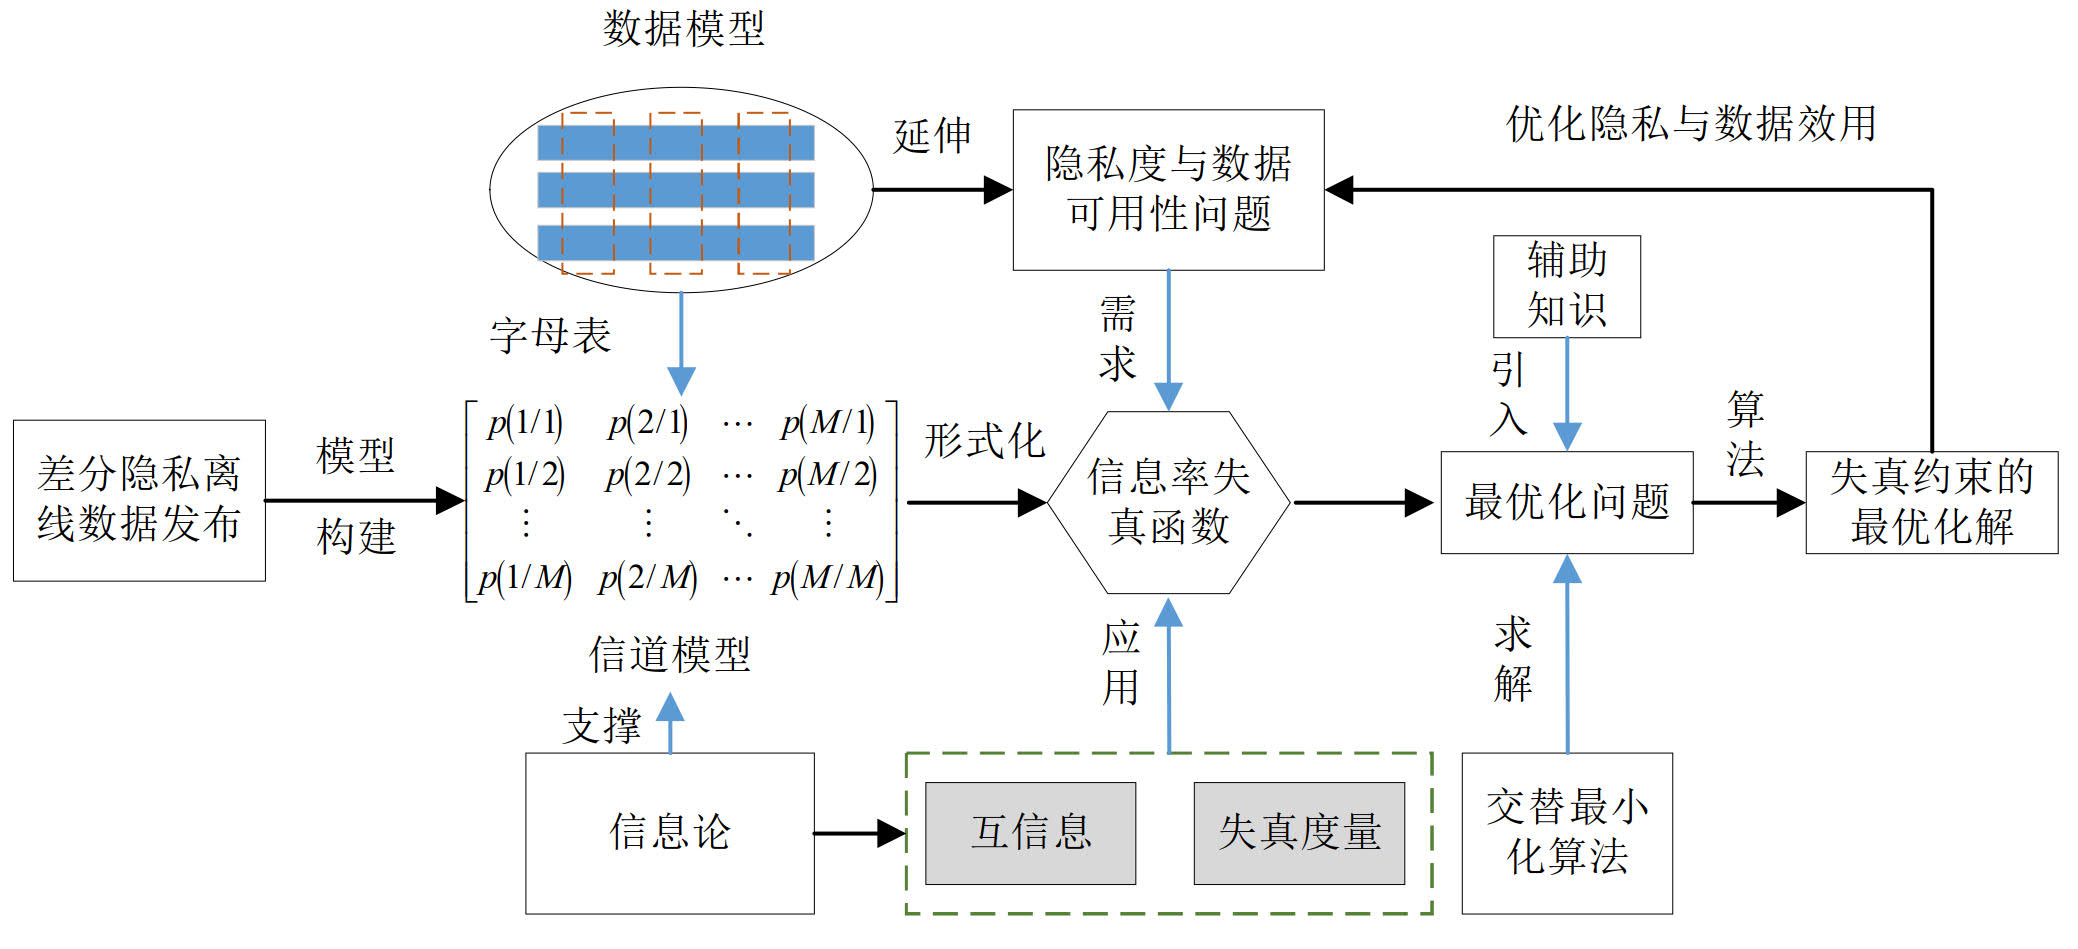
\includegraphics[width=5.0in]{chapter04/Figure4-1.jpg}
	\caption{权衡隐私与效用的差分隐私优化机制研究框架}
	\label{Fig:chapter05-1}
\end{figure}

在图\ref{Fig:chapter05-1}中,以差分隐私离线数据发布应用场景为立意的出发点,使用信息论、优化理论的方法解决数据发布中权衡隐私泄露与数据效用问题为研究目标。以下具体的介绍本章的研究思路:首先,通过分析差分隐私离线数据发布中原始数据扰动输出数据副本的处理流程,以数据模型、信道模型为基础,构建差分隐私信道模型。随后,从通信的角度给出本章信道模型的数学表达。以此为基础,针对隐私与效用的权衡问题,在熵与失真的度量基础上,将权衡隐私与效用的问题形式化为限失真约束条件下的最小化隐私信息泄露问题,给出互信息隐私优化模型,与著名的信息率失真函数具有相似的表述形式。其次,在差分隐私通信模型中引入含辅助背景知识攻击的敌手模型,将敌手拥有背景知识条件下的隐私与效用的权衡问题形式化为多约束条件的一个凸优化问题,给出条件互信息优化模型。最后,针对上述优化模型,研究模型的计算与算法求解问题。

\subsection{互信息隐私优化模型}\label{subsec:chapter05-mi-optimazation}
基于信息熵的度量模型及方法,互信息量度量差分隐私数据发布的隐私泄露,期望失真量化发布数据与原始数据的失真程度,也即是数据的可用性。直观上理解,差分隐私数据发布中的隐私泄露与数据效用是极大极小的矛盾问题。依据隐私保护中的隐私与效用原则\cite{sankar2013utility},权衡隐私与数据效用属于最优性均衡解决的问题。以此为理论的出发点,在限定数据可用性约束的前提下,利用隐私-失真函数形式化表述权衡问题为如下的优化模型$1$的形式。

\textbf{模型1:}差分隐私信道模型$\mathcal{Q}:\mathcal{X}\times \mathcal{\hat{X}}\rightarrow \mathbb{R}^{+}$获得可达的最小互信息隐私泄露量,当且仅当对于给定的数据分布$p(x)$,失真函数$d(x,\hat{x})$和数据质量约束$\mathbb{E}[d(X,\hat{X})]\leq \delta$,信道概率分布$q(\hat{x}|x)$是下述凸优化模型的最优解。
\begin{alignat}{2}
	R(\delta) & =\min_{q(\hat{x}|x)}I(X;\hat{X}) \nonumber \\
	\mbox{subject to} \quad
	& \sum_{x}\sum_{\hat{x}}p(x)q(\hat{x}|x)d(x,\hat{x})\leq  \delta \label{eq:chapter04-4-6}\\
	& \sum_{\hat{x}}q(\hat{x}|x)=1 \\
	& q(\hat{x}|x) \geq 0\label{eq:chapter04-4-8}
\end{alignat}
其中的$I(X;\hat{X})$和公式\ref{eq:chapter04-4-6}$\sim$\ref{eq:chapter04-4-8}分别是优化模型$1$的优化目标函数和约束条件,描述满足约束条件的$q(\hat{x}|x)$中寻找极小化$I(X;\hat{X})$的问题。

上述的优化模型$1$从隐私-失真的角度\cite{wang2016on}给出了权衡隐私与数据效用的基本优化模型,最小化信息率$R(\delta)$的形式化表述和Shannon信息论率失真函数\cite{cover2006elements}具有相同的表达形式,是关于信道条件概率分布$q(\hat{x}|x)$的最小值问题。在隐私保护中,最优化模型$1$在满足给定数据质量损失门限的前提条件下,求解最小化互信息隐私泄露的数据混淆机制,即信道条件概率分布。对此,文献\mycite{mir2012information,wang2016on}中已经给出了获得最优率失真的隐私机制依然提供一个确定等级差分隐私保护的结论。借用这个结论,通过上述模型$1$获得的信道概率满足$(\epsilon,\delta)$可达信道。
\subsection{条件互信息优化模型}\label{subsec:chapter-05-conditional-mioptimization}

上述优化模型$1$刻画了隐私与失真函数的关系,在隐私保护中具有广泛的应用\cite{wang2016on,sarwate2014a,mir2012information}。但是,上述模型中的隐私和失真函数没有考虑差分隐私离线数据发布场景中关联辅助背景知识对互信息隐私泄露的影响。实际应用中,由于隐私攻击者可能通过其它途径获取隐私关联数据,从而导致隐私泄露问题。本章中使用随机变量$Z$表示辅助的背景知识,并考虑由$Z$辅助识别的互信息隐私泄露问题。具体地说,依据隐私保护数据发布者和隐私攻击者对背景知识$Z$
的了解程度,将含背景知识的优化问题划分为如下的两种情形进行考虑:

%(1) 辅助背景知识$Z$是隐私保护数据发布者和隐私攻击者都知道的共同知识。在这种情况下,互信息的隐私度量$I(X;\hat{X})$改变为给定$Z$的条件下$X$和$\hat{X}$之间的条件互信息量$I(X;\hat{X}|Z)$。针对此,上述优化模型$1$中的最小化目标函数改变为求解变量$q(\hat{x}|x,z)$,使得条件互信息$I(X;\hat{X}|Z)$获得最小值。
%
%(2) 辅助背景知识$Z$是隐私攻击者可通过其它途径获得的外部关联数据,刻画了攻击者的能力。但是,数据发布者拥有一定有关辅助背景知识的统计信息,而未能精准的获得$Z$的具体数据细节。在这样的情形下,互信息的隐私度量$I(X;\hat{X})$改变为$X$和联合变量$\hat{X},Z$之间的互信息量$I(X;\hat{X},Z)$。针对此,上述优化模型$1$的最小化目标函数改变为求解条件概率$q(\hat{x},z|x)$使得$I(X;\hat{X},Z)$最小化。
\begin{itemize}[leftmargin=2em]
\item [(1)]辅助背景知识$Z$是隐私保护数据发布者和隐私攻击者都知道的共同知识。在这种情况下,互信息的隐私度量$I(X;\hat{X})$改变为给定$Z$的条件下$X$和$\hat{X}$之间的条件互信息量$I(X;\hat{X}|Z)$。针对此,上述优化模型$1$中的最小化目标函数改变为求解变量$q(\hat{x}|x,z)$,使得条件互信息$I(X;\hat{X}|Z)$获得最小值。

\item [(2)]辅助背景知识$Z$是隐私攻击者可通过其它途径获得的外部关联数据,刻画了攻击者的能力。但是,数据发布者拥有一定有关辅助背景知识的统计信息,而未能精准的获得$Z$的具体数据细节。在这样的情形下,互信息的隐私度量$I(X;\hat{X})$改变为$X$和联合变量$\hat{X},Z$之间的互信息量$I(X;\hat{X},Z)$。针对此,上述优化模型$1$的最小化目标函数改变为求解条件概率$q(\hat{x},z|x)$使得$I(X;\hat{X},Z)$最小化。
\end{itemize}

结合差分隐私离线数据发布应用场景中原始数据$X$到扰动数据$\hat{X}$之间的数据混淆过程,所表达出的隐私通信模型$X\xrightarrow{Q}\hat{X}$。考虑隐私攻击者可通过观察$\hat{X}$后,关联拥有的可用背景知识$Z$对原始数据$X$中的隐私信息进行推断攻击的敌手模型。本章中把隐私攻击者可以得到的背景知识$Z$考虑为仅攻击者拥有的知识。数据发布的混淆扰动过程表述为如图~\ref{Fig:chapter05-2}所示的隐私通信模型。
\begin{figure}[htbp]
	\centering
	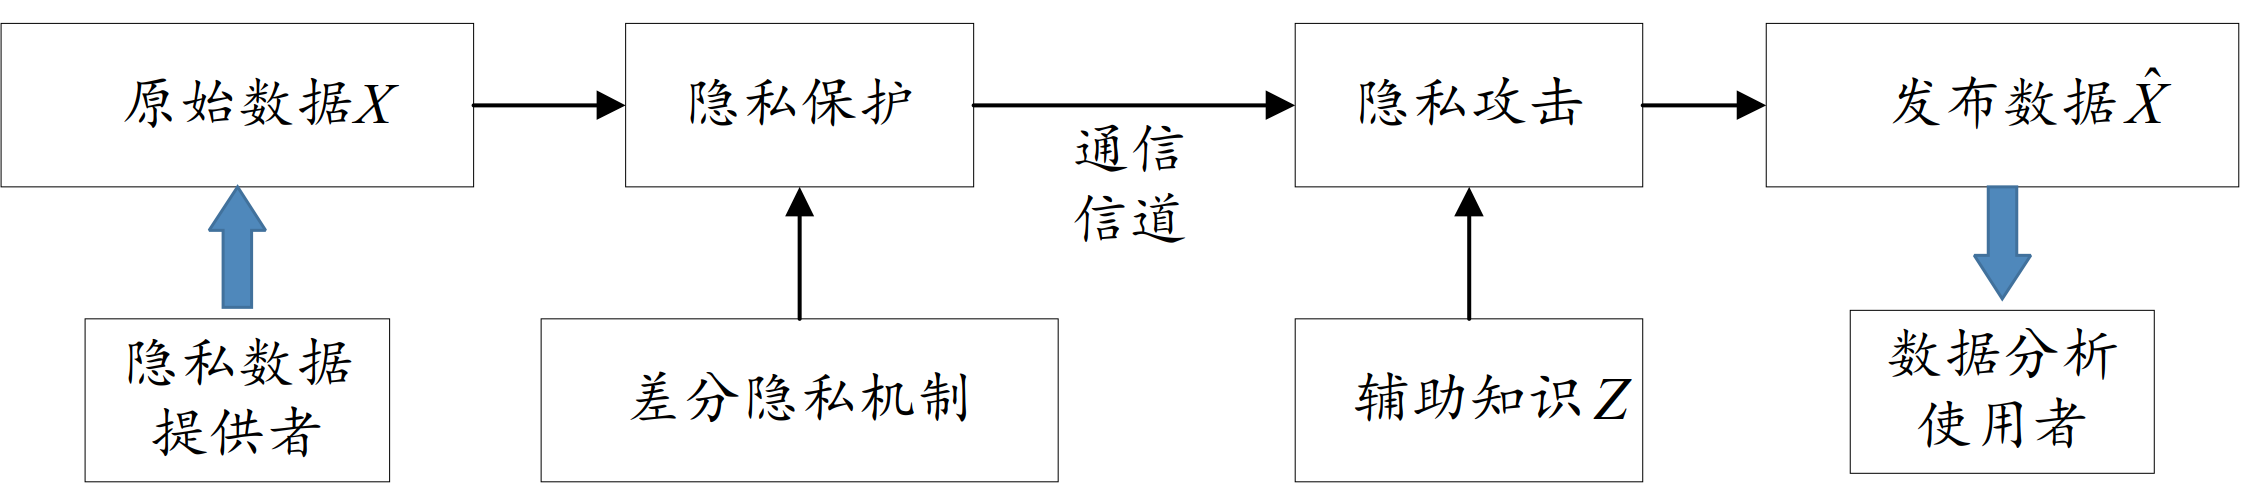
\includegraphics[width=5.0in]{chapter04/Figure2.png}
	\caption{含有背景知识攻击的差分隐私通信模型}
	\label{Fig:chapter05-2}
\end{figure}

为了更好的说明上图\ref{Fig:chapter05-2}中隐私攻击者具有关联辅助背景知识$Z$对互信息隐私泄露风险的影响,首先从理论上给出下述定理\ref{theorem:5.1}。
\begin{theorem} \label{theorem:5.1}随机变量$X$与$\hat{X},Z$的联合互信息量$I(X;\hat{X},Z)$不小于互信息$I(X;\hat{X})$。
\end{theorem}
\textbf{证明定理\ref{theorem:5.1}:}由随机变量$X$和$X,Z$联合的互信息量定义,则有
\begin{alignat}{2}
	I(X;\hat{X},Z) & =\sum_{x}\sum_{\hat{x}}\sum_{z}p(x,\hat{x},z)\log \frac{q(x|\hat{x},z)}{p(x)} \\
	 & = \sum_{x}\sum_{\hat{x}}\sum_{z}p(x,\hat{x},z)\log \left( \frac {q(x|\hat{x},z)}{q(x|\hat{x})}\cdot \frac{q(x|\hat{x})}{p(x)} \right)\\
	 & = \sum_{x}\sum_{\hat{x}}p(x,\hat{x})\log \frac{q(x|\hat{x})}{p(x)} \nonumber \\
	 & +\sum_{x}\sum_{\hat{x}}\sum_{z}p(x,\hat{x},z)\log \frac{q(x|\hat{x},z)}{q(x|\hat{x})}\\
	 & = I(X;\hat{X})+I(X;Z|\hat{X})\\
	 & \geq I(X;\hat{X})
\end{alignat}
易知,$I(X;\hat{X},Z)$是互信息$I(X;\hat{X})$和条件互信息$I(X;Z|\hat{X})$之和。因为平均互信息的非负性,则有结论成立。

基于上述互信息隐私泄露量的分析,拥有背景知识$Z$相对于$I(X;\hat{X})$可增加隐私泄露量。以此为基础,接下来将差分隐私数据发布中隐私攻击者拥有背景知识$Z$的最小化互信息隐私泄露问题定义为

\begin{definition}对于给定$X$的失真函数$d(x,\hat{x})$,差分隐私信道模型$\mathcal{Q}:\mathcal{X}\times \mathcal{\hat{X}}\rightarrow \mathbb{R}^{+}$,在满足$\mathbb{E}[d(X,\hat{X})]\leq \delta$的约束下,隐私信道获得的最小互信息隐私泄露量为信息率$R_{z}(\delta)$。其中,$R_{z}(\delta)$为下述最优化模型$2$的最优值。
\end{definition}

\textbf{模型2:}对于数据$X$的失真函数$d(x,\hat{x})$,在$Z$的条件下,数据质量满足限失真门限$\delta$的约束,条件概率$q(\hat{x},z|x)$是获得最小化互信息隐私泄露$R_{z}(\delta)$ 的最优点,即是下述优化问题的最优解。
\begin{alignat}{2}%\label{eq:chapter05-model2}
	R_{z}(\delta) & =\min_{q(\hat{x},z|x)}I(X;\hat{X},Z) \nonumber \\
	\mbox{subject to} \quad
	& \sum_{x}\sum_{\hat{x}}\sum_{z}p(x)q(\hat{x},z|x)d(x,\hat{x})\leq  \delta \label{eq:chapter04-14}\\
	& \sum_{\hat{x}}\sum_{z}q(\hat{x},z|x)=1\\
	& q(\hat{x},z|x) \geq 0\label{eq:chapter04-16}
\end{alignat}
其中$I(X;\hat{X},Z)=\sum_{x,\hat{x},z}p(x,\hat{x},z)\log \frac{q(\hat{x},z|x)}{p(\hat{x},z)}$和公式\ref{eq:chapter04-14}$\sim$\ref{eq:chapter04-16}分别为目标函数和约束条件。

上述最优化模型$2$是互信息隐私泄露$I(X;\hat{X},Z)$关于条件概率分布$q(\hat{x},z|x)$的最小值求解问题。换句话表述,上述优化模型$2$的最优解$q(\hat{x},z|x)$就是在数据质量损失约束条件下,使得互信息量$I(X;\hat{X},Z)$获得极小值。

\section{差分隐私数据发布机制与优化}\label{chapter05-optimazation-mechanism}

本节中针对上述优化模型$2$,利用Lagrange对偶函数的方法对权衡隐私与效用的优化模型进行求解,给出KKT条件的参量表达式。然后,针对直接计算最优条件概率分布的困难性问题,基于Blahut-Arimoto算法给出了差分隐私数据发布场景中计算最优信道条件概率分布的迭代算法。

\subsection{优化模型最优解}

借鉴率失真函数的求解方法,最优化模型$2$是满足期望失真约束和条件概率分布约束条件下,有关凸目标函数的一个标准最小化问题。对其利用Lagrange乘子法进行求解,首先构造以下泛函$L(q)$
\begin{alignat}{2}
	L(q) & =\sum_{x}\sum_{\hat{x},z}q(\hat{x},z|x)\log \frac{q(\hat{x},z|x)}{q(\hat{x},z)} \nonumber \\
	  & + \lambda \sum_{x}\sum_{\hat{x},z}p(x)q(\hat{x},z|x)d(x,\hat{x}) \\
	& +\sum_{x}\nu (x)\sum_{\hat{x},z}q(\hat{x},z|x) \nonumber
\end{alignat}

然后,对构造的$L(q)$关于$q(\hat{x},z|x)$求偏导数,并令$\frac{\partial L(q)}{\partial q(\hat{x},z|x)}=0$得到如下含有拉格朗日乘子参数$\lambda$的表达式
\begin{alignat}{2}
	\frac{\partial L(q)}{\partial q(\hat{x},z|x)} & =p(x)\log \frac{q(\hat{x},z|x)}{q(\hat{x},z)}+p(x)
	-\sum_{x'}p(x')q(\hat{x},z|x')\frac{1}{q(\hat{x},z)}p(x) \nonumber \\
	 & + \lambda p(x)d(x,\hat{x}) \\
	& +\nu (x) \nonumber \\
	& = 0 \nonumber
\end{alignat}
由于先验概率分布$p(x)\geq 0$,利用KKT条件可以计算得到使得互信息最小化的条件概率$q(\hat{x},z|x)$参量表达式
\begin{equation}\label{eq:chapter05-pdf}
	q(\hat{x},z|x)=\frac{q(\hat{x},z)e^{-\lambda d(x,\hat{x})}}{\sum_{\hat{x},z}q(\hat{x},z)e^{-\lambda d(x,\hat{x})}}
\end{equation}

然而,通过联合方程组的方式直接解出最优输出分布仍然比较困难。针对这个计算的困难问题,Blahut和Arimoto\cite{arimoto1972an,blahut1972computation}提出了计算率失真函数的迭代求解算法,该算法是两个概率分布凸集之间计算最小相对熵距离的一种特殊情况\cite{cover2006elements}。已经证明算法在两个概率分布凸集之间交替最小化相对熵距离的计算过程中存在一个极限,收敛到相对熵距离最小值。基于此,求解率失真$R(\delta)$需要将率失真函数改写为两个集合之间相对熵距离最小化的形式。为了将其改进应用到优化模型$2$的求解计算中,以下给出计算的预处理过程。

\subsection{交替最小化算法}
对于两个给定凸集$A$和$B$以及欧几里得范数距离,目标是计算集合$A$和$B$之间的最小欧氏距离。利用交替最小化的思想,首先,选择任意的$a \in A$ ,计算$b \in B$满足~$\min \parallel a-b\parallel_{2}$。然后固定~$b$,在集合$A$中计算欧式距离和$b$最近的元素。重复上述计算过程,随着重复次数增加,特定的距离度量收敛于两个集合的最小值\cite{cover2006elements}。特别地,如果上述是在两个概率分布集合$A$和$B$之间的相对熵(Kullback-Leibler,KL) 距离度量中,最小化距离的算法将收敛到$A$和$B$之间的最小相对熵\cite{csiszar1984information}。

本章中,基于上述最小化算法的交替计算过程对提出的优化模型进行求解。首先,需要将其改写为相对熵距离在两个概率分布集合之间双重最小化的形式。为此,给出以下引理\ref{lemma:chapter05-1}。
\begin{lemma}\label{lemma:chapter05-1}设$p(x)q(\hat{x},z|x)$是给定的联合分布,使得最小化相对熵$D(p(x)q(\hat{x},z|x)\parallel p(x)r(\hat{x},z))$~的分布$r(\hat{x},z)$是对应于条件概率$q(\hat{x},z|x)$的边缘分布$r^*(\hat{x},z)$,也即是
	\begin{equation}\label{lemma5.1}
		D_{KL}(p(x)q(\hat{x},z|x)\parallel p(x)r^*(\hat{x},z))=\min_{r(\hat{x},z)}D_{KL}(p(x)q(\hat{x},z|x)\parallel p(x)r(\hat{x},z))
	\end{equation}
	其中,$r^*(\hat{x},z)=\sum_{x}p(x)q(\hat{x},z|x)$。
\end{lemma}
\textbf{证明引理\ref{lemma:chapter05-1}:}根据相对熵$D_{KL}(\cdot||\cdot)$的定义,构造
\begin{alignat}{2}
	D_{KL}\left( p(x)q(\hat{x},z|x)\parallel p(x)r(\hat{x},z)\right)
	 & -D_{KL}\left(p(x)q(\hat{x},z|x)\parallel p(x)r^{*}(\hat{x},z)\right) \\
	 & =\sum_{x,\hat{x},z}p(x)q(\hat{x},z|x)\log \frac{p(x)q(\hat{x},z|x)}{p(x)r(\hat{x},z)}\\
	 & - \sum_{x,\hat{x},z}p(x)q(\hat{x},z|x)\log \frac{r^*(\hat{x},z)}{r(x,z)}\\
	 & = \sum_{x}\sum_{\hat{x}}p(x,\hat{x})\log \frac{q(x|\hat{x})}{p(x)} \nonumber \\
	 &=\sum_{\hat{x},z}r^*(\hat{x},z)\log \frac{r^*(\hat{x},z)}{r(x,z)}\\
	 & =D_{KL}\left(r^*(\hat{x},z)\parallel r(\hat{x},z)\right)
\end{alignat}
由于相对熵的非负性质,则有$D_{KL}\left(r^*(\hat{x},z)\parallel r(\hat{x},z)\right)\geq 0$的结论。当且仅当,$r^*(\hat{x},z)= r(\hat{x},z)$ 时等号成立。

基于引理\ref{lemma:chapter05-1}和$I(X;\hat{X},Z)=\sum_{x}\sum_{\hat{x}}\sum_{z}p(x,\hat{x},z)\log \frac{q(\hat{x},z|x)}{p(\hat{x},z)}$的计算公式,可以将上述优化模型$2$中的最优化目标函数$I(X;\hat{X},Z)$表述为一个具有相对熵距离的双重最小化问题的形式,则有
\begin{alignat}{2}
& \min_{q(\hat{x},z|x):\sum_{x,\hat{x},z}p(x)q(\hat{x},z|x)d(x,\hat{x})\leq  \delta}\sum_{x,\hat{x},z} p(x,\hat{x},z)\log \frac{q(\hat{x},z|x)}{p(\hat{x},z)}\\
=\min_{r(\hat{x},z)}&\min_{q(\hat{x},z|x):\sum_{x,\hat{x},z}p(x)q(\hat{x},z|x)d(x,\hat{x})\leq  \delta}\sum_{x,\hat{x},z}p(x)q(\hat{x},z|x)\log \frac{q(\hat{x},z|x)}{r(\hat{x},z)}\label{eq:chapter05-double}
\end{alignat}

针对上式~\ref{eq:chapter05-double}中的双重最小化问题,利用交替最小化算法进行计算近似最优解。如果集合$A$为边际分布$p(x)$满足期望失真门限的所有联合概率分布 $p(x,\hat{x},z)$的集合,$B$为乘积分布$p(x)r(\hat{x},z)$构成的集合,则对于任意的分布$r(\hat{x},z)$,上述公式\ref{eq:chapter05-double}中的双重最小化可以表述为如下公式\ref{eq:chapter04-1-28}的形式,

\begin{equation}\label{eq:chapter04-1-28}
	\min_{q(\hat{x},z|x):\sum_{x,\hat{x},z}p(x)q(\hat{x},z|x)d(x,\hat{x})\leq  \delta } I(X;\hat{X},Z)=\min_{q \in B}\min_{p \in A} D_{KL}(p\parallel q)
\end{equation}

基于上述方法将优化模型$2$中的问题转变为了两个概率分布集合之间计算最小相对熵距离的双重最小化问题。然后,借鉴计算率失真函数的交替最小化算法\cite{csiszar1984information,csiszar1974on},设计本章中对优化模型$2$求解的近似算法。以下\ref{sec:chapter04-algorithm}节详细阐述本章中最优信道模型概率分布的迭代近似计算过程。

\subsection{优化模型迭代算法}\label{sec:chapter04-algorithm}

针对上述优化模型2中所描述的具有多约束条件的凸优化问题,本节中采用两个概率分布集合之间相对熵距离双重最小化的迭代计算方法进行求解。基于Blahut-Arimoto算法作为基础设计求解优化模型计算信道条件概率分布的迭代算法。算法接受预设参数输入,包括Lagrange乘子$\lambda$、数据先验分布$p(x)$、汉明失真$d(x,\hat{x})$和收敛阈值门限$T$。具体的迭代计算过程包含有以下几个步骤。

(1) 首先,初始化算法输出的联合概率分布$r_0(\hat{x},z)$为均匀分布。

(2) 其次,利用Lagrange 乘子法求解得到的公式~\ref{eq:chapter05-pdf}~的条件概率表达式计算条件概率分布$q_0(\hat{x},z|x)$和互信息量$I(X;\hat{X},Z)$。然后,基于引理\ref{lemma:chapter05-1}为基础,计算$r(\hat{x},z)=\sum_{x}p(x)q_0(\hat{x},z|x)$。

(3) 最后,重复上述计算步骤(2)直到互信息量收敛于阈值门限$T$。

上述迭代计算过程结束,算法输出可获得的最小互信息隐私泄露量以及条件概率分布$q(\hat{x},z|x)$ 和期望汉明失真。这个计算过程在算法\ref{alg:chapter05-1}中通过伪代码的形式给出了具体的描述。
\begin{algorithm}[htbp]
 \small
 \setstretch{1.2}
\caption{ 最小化互信息隐私泄露量}
\label{alg:chapter05-1}
\begin{algorithmic}[1]
\REQUIRE ~~\\
\begin{tabular}[t]{p{8mm}l}
 $\lambda$&:  Lagrange乘子\\
 $p(x)$&: 数据先验分布\\
 $d(x,\hat{x})$&: 汉明失真矩阵\\
 $T$&: 收敛门限阈值参数
\end{tabular}
\ENSURE ~~\\
\begin{tabular}[t]{p{8mm}l}
$q(\hat{x},z|x)$&: 条件概率分布\\
$MI^*$&: 最小的互信息泄露量$I(X;\hat{X},Z)$\\
$\bar{\delta}$&: 达到最小互信息时的期望失真度
\end{tabular}
\STATE 初始化$r_0(\hat{x},z)$为均匀分布
\STATE 计算$q_0(\hat{x},z|x)=\frac{r_0(\hat{x},z)e^{-\lambda d(x,\hat{x})}}{\sum_{\hat{x},z}r_0(\hat{x},z)e^{-\lambda d(x,\hat{x})}}$
\STATE $I_0\leftarrow $算法\ref{alg:chapter05-2}利用$p(x),q_0(\hat{x},z|x),r_0(\hat{x},z)$计算互信息/*子程序\ref{alg:chapter05-2}*/
\STATE 计算$r(\hat{x},z)=\sum_{x}p(x)q_0(\hat{x},z|x)$
\WHILE{true}
\STATE 计算$q(\hat{x},z|x)=\frac{r(\hat{x},z)e^{-\lambda d(x,\hat{x})}}{\sum_{\hat{x},z}r_0(\hat{x},z)e^{-\lambda d(x,\hat{x})}}$;
\STATE $I \leftarrow $算法\ref{alg:chapter05-2}利用$p(x),q(\hat{x},z|x),r(\hat{x},z)$
\IF{$I_0-I \leq T$}
\STATE $MI^* \leftarrow I$
\STATE 期望失真度$\bar{\delta}=\sum_{x,\hat{x},z}p(x)q(\hat{x},z|x)d(x,\hat{x})$
\RETURN $MI^*, q(\hat{x},z|x), \bar{\delta}$
\ELSE
\STATE $I_0 \leftarrow I$
\STATE $r(\hat{x},z)=\sum_{x}p(x)q(\hat{x},z|x)$
\ENDIF
\ENDWHILE
\end{algorithmic}
\end{algorithm}

上述算法\ref{alg:chapter05-1}中的步骤$3$利用算法\ref{alg:chapter05-2}进行互信息隐私泄露的计算。依据$X$与$X,\hat{Z}$的联合互信息计算公式
\begin{equation}
	I(X;\hat{X},Z)=\sum_{x,\hat{x},z}p(x)q(\hat{x},z|x) \log \frac{q(\hat{x},z|x)}{q(\hat{x},z)}
\end{equation}
得到信息泄露量,具体的计算细节在算法\ref{alg:chapter05-2}中给出描述。

\begin{algorithm}[htb]
 \small
 \setstretch{1.2}
\caption{ 计算互信息隐私泄露量}
\label{alg:chapter05-2}
\begin{algorithmic}[1]
\REQUIRE ~~\\
\begin{tabular}[t]{p{8mm}l}
 $p(x)$&: 数据先验分布\\
 $q(\hat{x},z|x)$&: 条件概率分布\\
 $r(\hat{x},z)$&: 联合概率分布
\end{tabular}
\ENSURE ~~\\
\begin{tabular}[t]{p{8mm}l}
$MI$&: 平均互信息隐私泄露量
\end{tabular}
\STATE 初始化设置$MI = 0$
\FOR{循环遍历$X,\hat{X}$,以及$Z$取值空间,$i \in |\mathcal{X}|, j \in |\mathcal{\hat{X}}|,k \in |\mathcal{Z}|$}
\STATE $MI \leftarrow \sum p(x_i)q(\hat{x}_j,z_k|x_i) \log \frac{q(\hat{x}_j,z_k|x_i)}{r(\hat{x}_j,z_k)}$
\ENDFOR
\RETURN $MI$;
\end{algorithmic}
\end{algorithm}

基于上述算法\ref{alg:chapter05-1}可以得到最小互信息隐私泄露量时的信道条件概率分布$q(\hat{x},z|x)$。然而,根据差分隐私定义\ref{def:chapter05-dp},隐私保护的不可区分度和条件概率$q(\hat{x}|x)$相关。由此,首先需要利用条件概率公式计算联合概率分布$p(x,\hat{x},z)$,进而基于联合概率分布,关于辅助背景知识$Z$计算边缘概率分布$q(x,\hat{x})$。其次,以数据先验概率分布$p(x)$为基础,计算得到隐私机制的信道条件概率分布$q(\hat{x}|x)$。基于互信息度量是平均意义上的隐私泄露量,但是,率失真函数方法获得的隐私机制依然能够提供一个确定等级的差分隐私保护\cite{wang2016on,mir2012information}。以此为基础依据,针对信道条件概率分布$q(\hat{x}|x)$根据定义\ref{def:chapter05-dp}利用公式\ref{eq:chapter05-epsilon}计算差分隐私的预算参数,具体过程如算法\ref{alg:chapter05-3}中伪代码描述。
\begin{algorithm}[htb]
\caption{信道条件概率和隐私预算参数}
\label{alg:chapter05-3}
 \small
 \setstretch{1.2}
\begin{algorithmic}[1]
\REQUIRE ~~\\
\begin{tabular}[t]{p{8mm}l}
 $q(\hat{x},z|x)$&: 条件概率分布\\
 $p(x)$&: 数据先验分布
\end{tabular}
\ENSURE ~~\\
\begin{tabular}[t]{p{8mm}l}
$q(\hat{x}|x)$&: 信道条件概率\\
$\epsilon^*$  &: 差分隐私预算参数
\end{tabular}
\STATE 计算边缘分布$q(x,\hat{x})=\sum_{z}p(x)q(\hat{x},z|x)$
\STATE 计算条件概率分布$q(\hat{x}|x)=\frac{q(x,\hat{x})}{p(x)}$
\FOR{循环遍历$X,\hat{X}$,$i \in |\mathcal{X}|, j \in |\mathcal{\hat{X}}|$}
\STATE 求解$\epsilon^* = \min \left\{\log \max \left[\frac{p(\hat{x}_j|x_i)}{p(\hat{x}_j|x'_i)}\right]\right\}$
\ENDFOR
\RETURN $q(\hat{x}|x)$,$\epsilon^*$
\end{algorithmic}
\end{algorithm}

\begin{remark}
	{\em 以下给出算法的计算复杂性分析。上述迭代最小化算法\textup{\ref{alg:chapter05-1}}的基本操作是计算$q(\hat{x},z|x)$、$r(\hat{x},z)$及互信息量$I(X;\hat{X},Z)$。算法的每一轮计算过程中,算法\textup{\ref{alg:chapter05-1}}的第$6$行中$(\hat{x},z)$的计算需要进行$O\left(|\hat{X}||Z|\right)$ 次基本运算。由此,对所有的$x$计算条件概率分布需要的基本运算次数是$O\left(|X||\hat{X}||Z|\right)$。其次,算法\textup{\ref{alg:chapter05-1}}的第$7$ 行中计算互信息隐私量也是需要$O\left(|X||\hat{X}||Z|\right)$次基本运算操作。最后,第$14$行中联合概率分布$r(\hat{x},z)$的计算,对每一个变量$x$的基本运算复杂度是$O\left(|\hat{X}||Z|\right)$。因此,计算$r(\hat{x},z)$ 的复杂度是$O\left(|X||\hat{X}||Z|\right)$。综合以上分析,算法\textup{\ref{alg:chapter05-1}}的总体计算时间复杂度为问题规模源字母表空间、再生字母表空间及辅助背景知识空间大小的函数,也即是$O\left(|X||\hat{X}||Z|\right)$。}
\end{remark}
\section{实验与分析}\label{chapter04-experiment}
本节中针对上述优化模型所设计的迭代算法进行实验仿真,从互信息隐私泄露和期望失真的角度展示了具体的实验结果。以下具体介绍实验环境与实验结果。
\subsection{实验设置}
本章中的算法使用Java程序语言及第三方Math数学工具包编程实现,利用公开数据集MovieLens和Adult在Intel Core i5-6300U,2.4GHz,4G运行Windows10 X64 操作系统的个人PC上运行算法。以下简单给出基础数据集的说明。
\begin{itemize}
\item [(1)]MovieLens\footnote{https://grouplens.org/datasets/movielens/}是用户电影评分数据集,其中包含了$943$个用户对$1682$部电影的$100000$ 个评分数据。评分数据中的评分等级rating是一个范围在$1 \sim 5$的整数。

\item [(2)]机器学习的Adult数据集原始具有$15$个属性,删除丢失数据项的记录后,实际得到了$30162$个有效元组。本节实验中选择 Marital-status (婚姻状态)、Occupation(职业)类别型变量进行实验分析。
\end{itemize}
\subsection{实验分析}

实验分析环节,针对本章中隐私攻击者有或无辅助背景知识的优化模型1和优化模型2,分别给出了真实数据集上的实验分析。

\textbf{(1)} 针对差分隐私数据发布中无辅助背景知识的优化模型$1$,选择MovieLens用户电影评分数据集中编号$785$的评分数据,各项评分等级的概率分布是$p(x)=\{0.0513,0.1538,\\0.4872,0.2051,0.1026\}$,信息熵$H(x)=1.9464$。然后,利用汉明失真测量建立汉明失真矩阵。进一步,选择$\lambda$乘子取值区间$\lambda \in [0.6,10]$和收敛阈值门限$T=10^{-8}$,计算$\lambda$选取不同取值时,优化模型$1$对应的隐私机制的互信息隐私泄露量、期望失真程度和满足差分隐私的预算参数。
\begin{figure}[htbp]
\centering
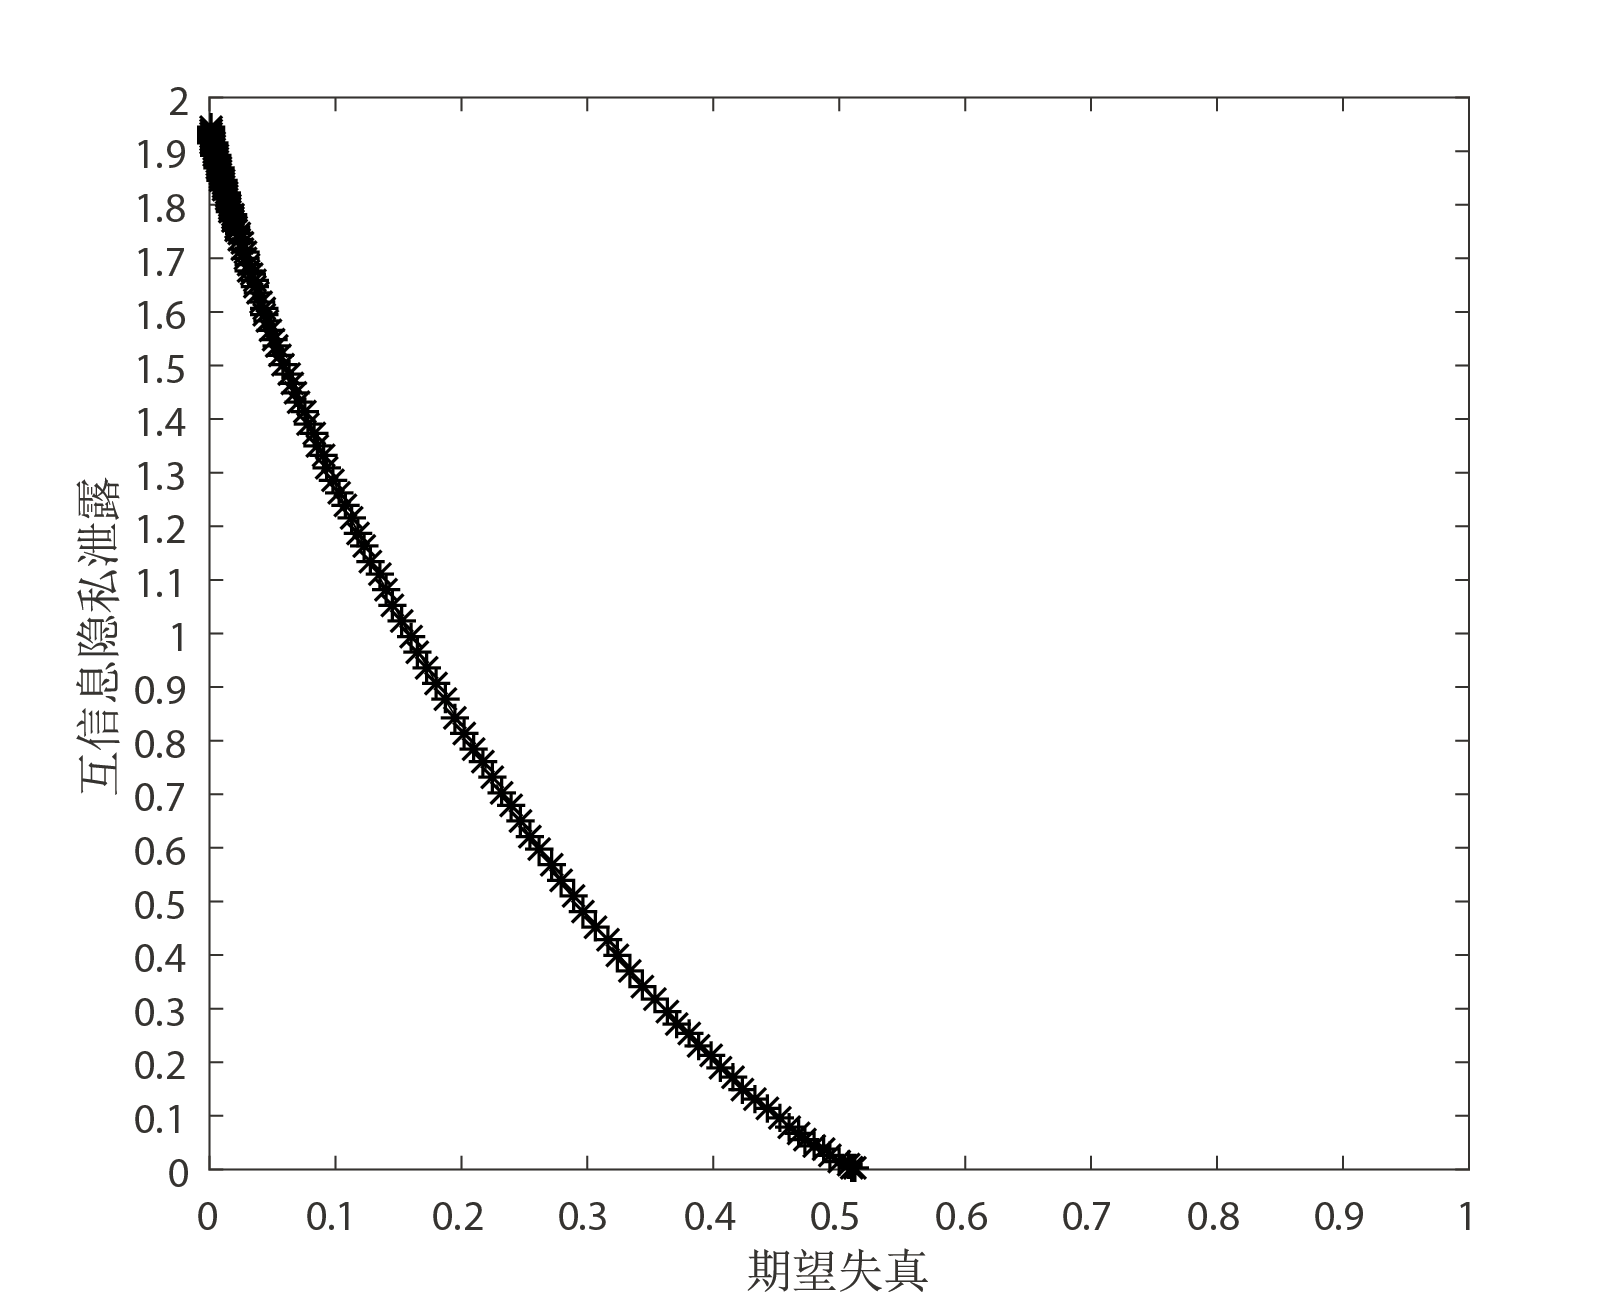
\includegraphics[width=3.5in]{chapter04/Figure3.png}
\caption{MovieLens数据集评分的率失真曲线}
\label{Fig:chapter05-3}
\end{figure}

图\ref{Fig:chapter05-3}所示为MovieLens电影评分数据集的期望汉明失真和互信息之间的率失真曲线。图中显示,随着期望失真度逼近于$0$,互信息度量的隐私泄露逼近于信息熵。此外,当期望失真度大于$0.5$,互信息隐私泄露量趋近于$0$,这个变化过程表现出了互信息隐私量和期望失真之间的变化关系。
\begin{figure}[htbp]
\centering
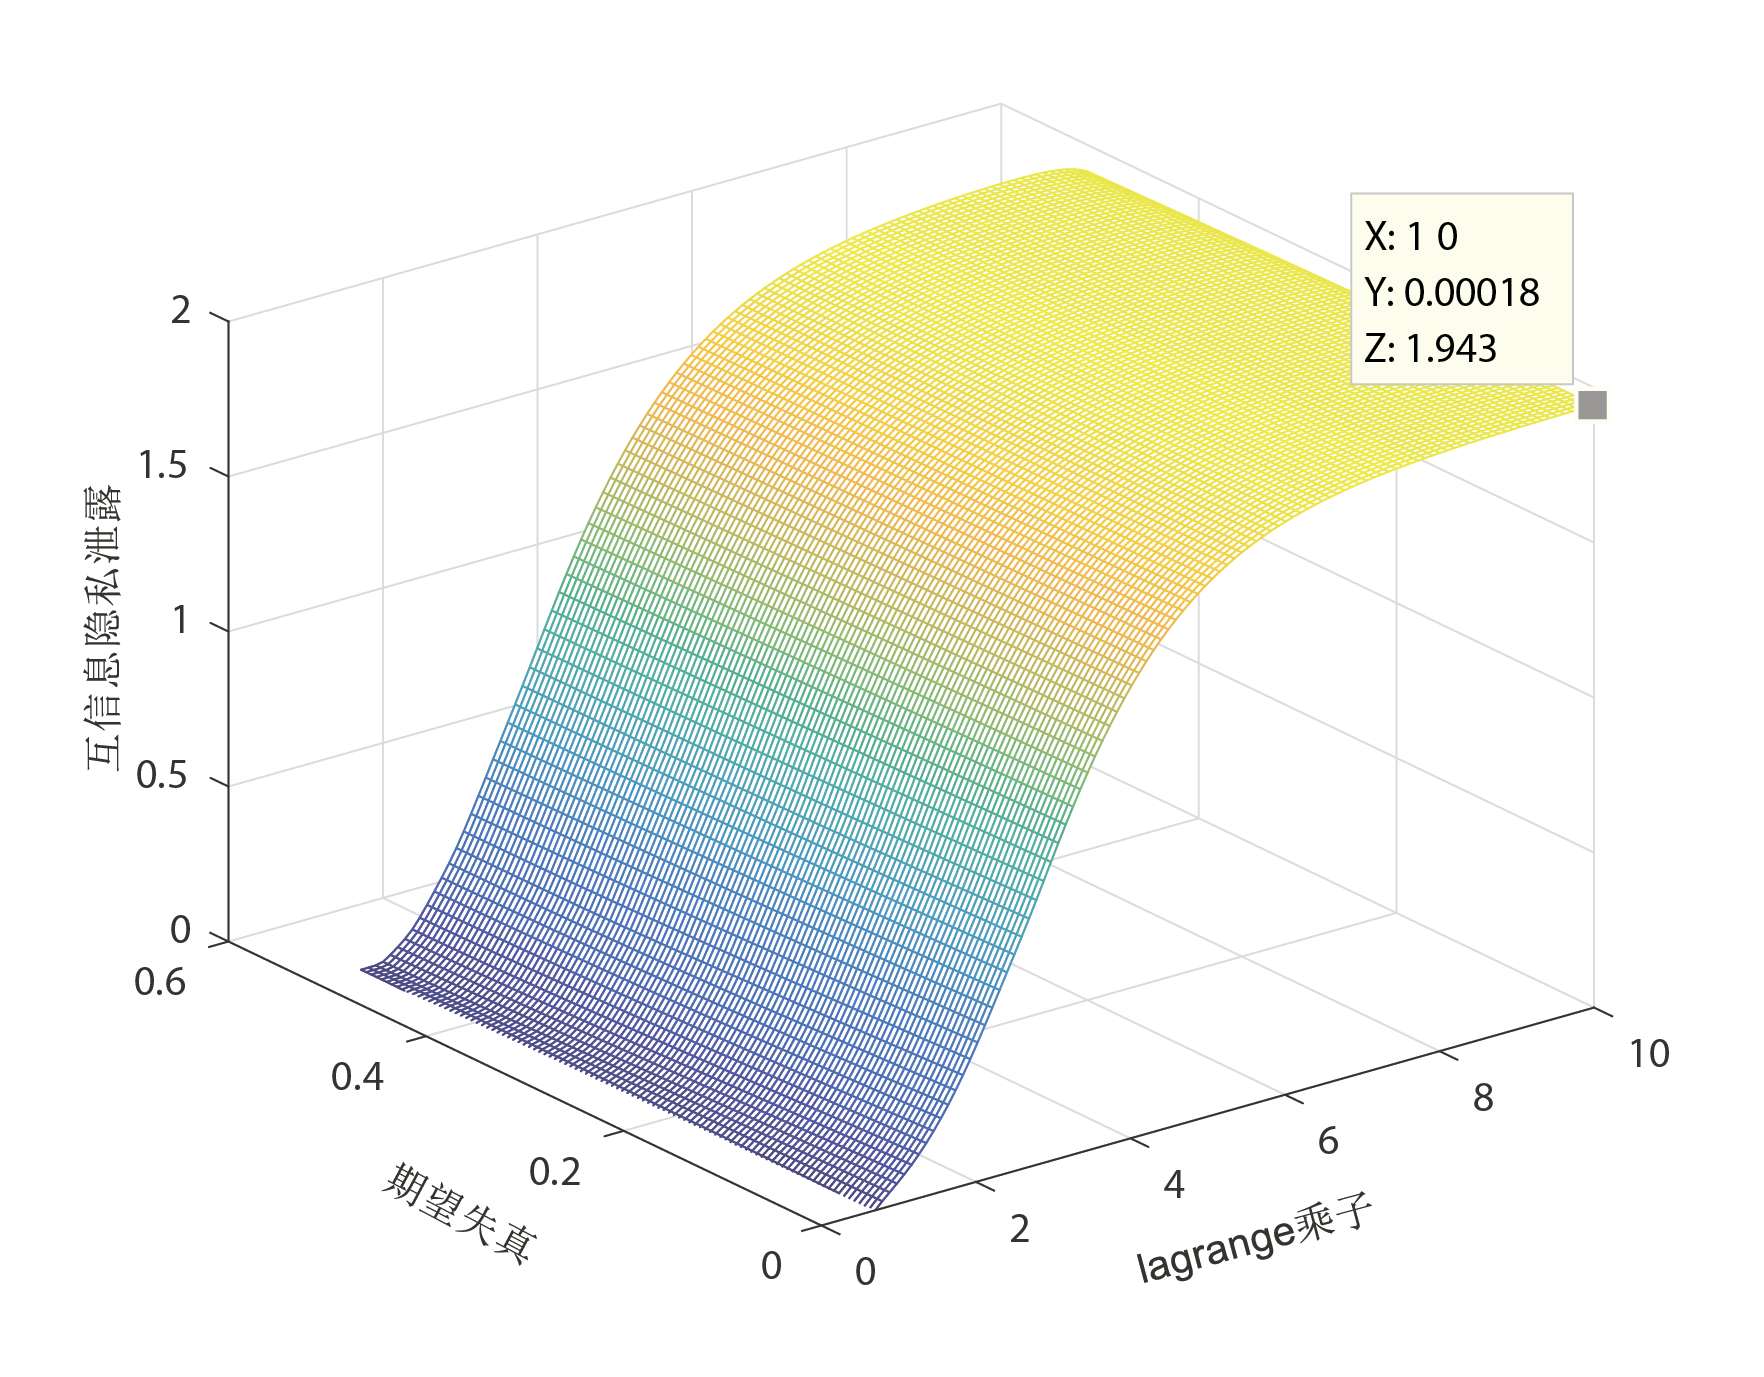
\includegraphics[width=3.5in]{chapter04/Figure4.png}
\caption{ 期望失真、互信息隐私和拉格朗日乘子关系}
\label{Fig:chapter05-4}
\end{figure}
\begin{figure}[htbp]
\centering
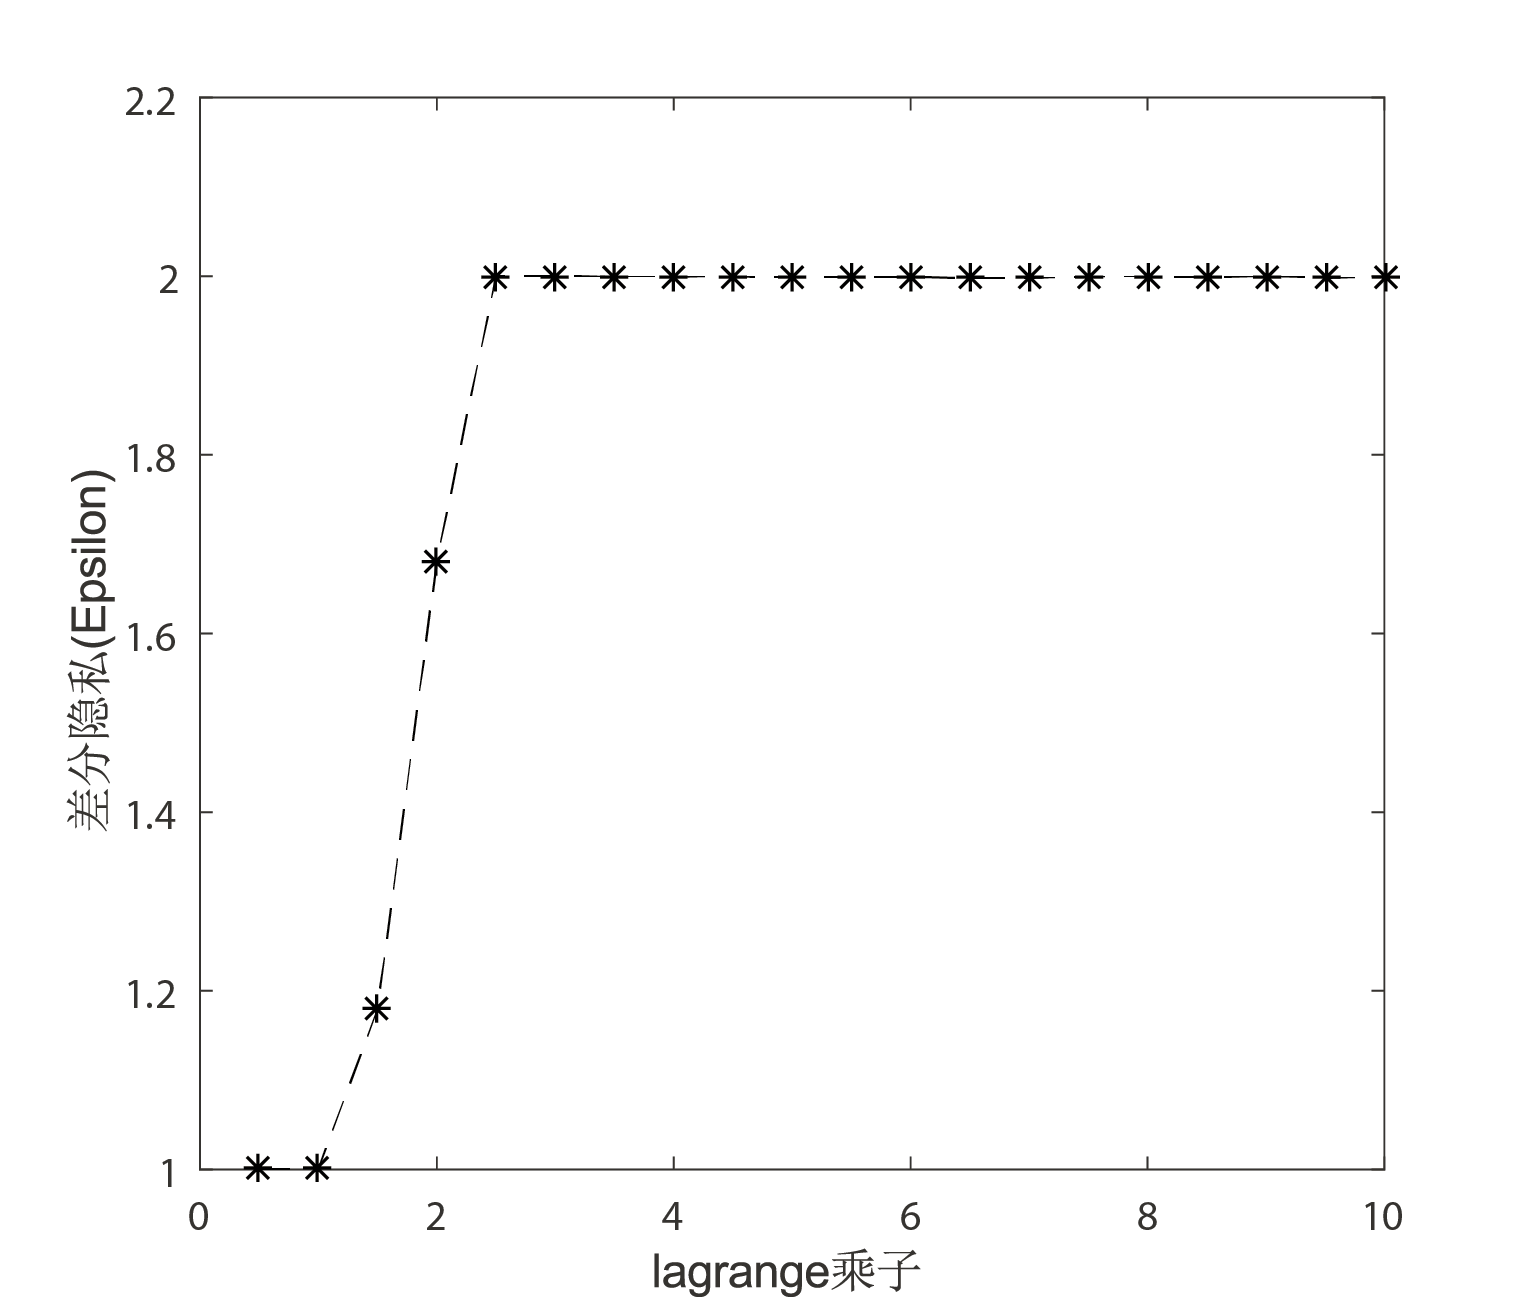
\includegraphics[width=3.5in]{chapter04/Figure5.png}
\caption{拉格朗日乘子与差分隐私参数关系}
\label{Fig:chapter05-5}
\end{figure}

除此之外,实验分析了Lagrange乘子$\lambda$变化对所计算的隐私机制在期望失真和互信息隐私方面的影响。当$T=10^{-8}$时,$\lambda$和互信息隐私、期望失真之间的关系表达为三维图\ref{Fig:chapter05-4}。从图中显示的结果分析,在$\lambda=10.0$时,互信息量$1.943$接近于信源熵$1.9464$,对应的期望失真$0.00018$逼近于$0$,这个关系与图\ref{Fig:chapter05-3}中的曲线图显示结果相吻合。

优化模型迭代求解的算法中$\lambda$和$T$通过影响算法输出的信道条件概率分布进而影响差分隐私保护等级,即隐私预算参数。为了量化隐私机制的不可区分度给出了实验分析。图\ref{Fig:chapter05-5}中展示了信道条件概率满足差分隐私预算参数的曲线(以$\ln$为单位)。从图中所示结果分析,随着$\lambda$变大隐私参数趋近于稳定。结合图\ref{Fig:chapter05-4}和图\ref{Fig:chapter05-5}的结果可知,$\lambda$增加使得互信息隐私量变大,隐私保护的强度变弱,但是,$\lambda$的增加对互信息隐私的影响变弱,使得隐私保护强度无明显变化。


\textbf{(2)} 针对差分隐私数据发布应用中隐私攻击者具有辅助背景知识的优化模型$2$。利用Adult数据集进行实验分析,首先,选择数据集中的Marital-status(婚姻状态)属性,其是类别型属性,域值具有$7$个不同的取值,实验中将其作为发布时的原始数据$X$。其次,由于数据集中Occupation(职业)和Marital-status之间的数据关联,实验中选择Occupation属性,属性域具有$14$个不同的取值,将其考虑为辅助的背景知识$Z$。基于上述数据进行模型$2$的分析,首先,原始数据$X$的概率分布$p(x)=\{0.1386,0.0007,0.4668,0.0127,0.322,0.0312,0.0273\}$,信息熵$H(X)=1.82$。随后,对于类别型属性假设原始与混淆扰动数据域相同,建立汉明失真矩阵。进一步,选择$\lambda \in [0.5,1.0]$,$T=10^{-8}$利用算法\ref{alg:chapter05-1}进行实验。
\begin{figure}[htbp]
\centering
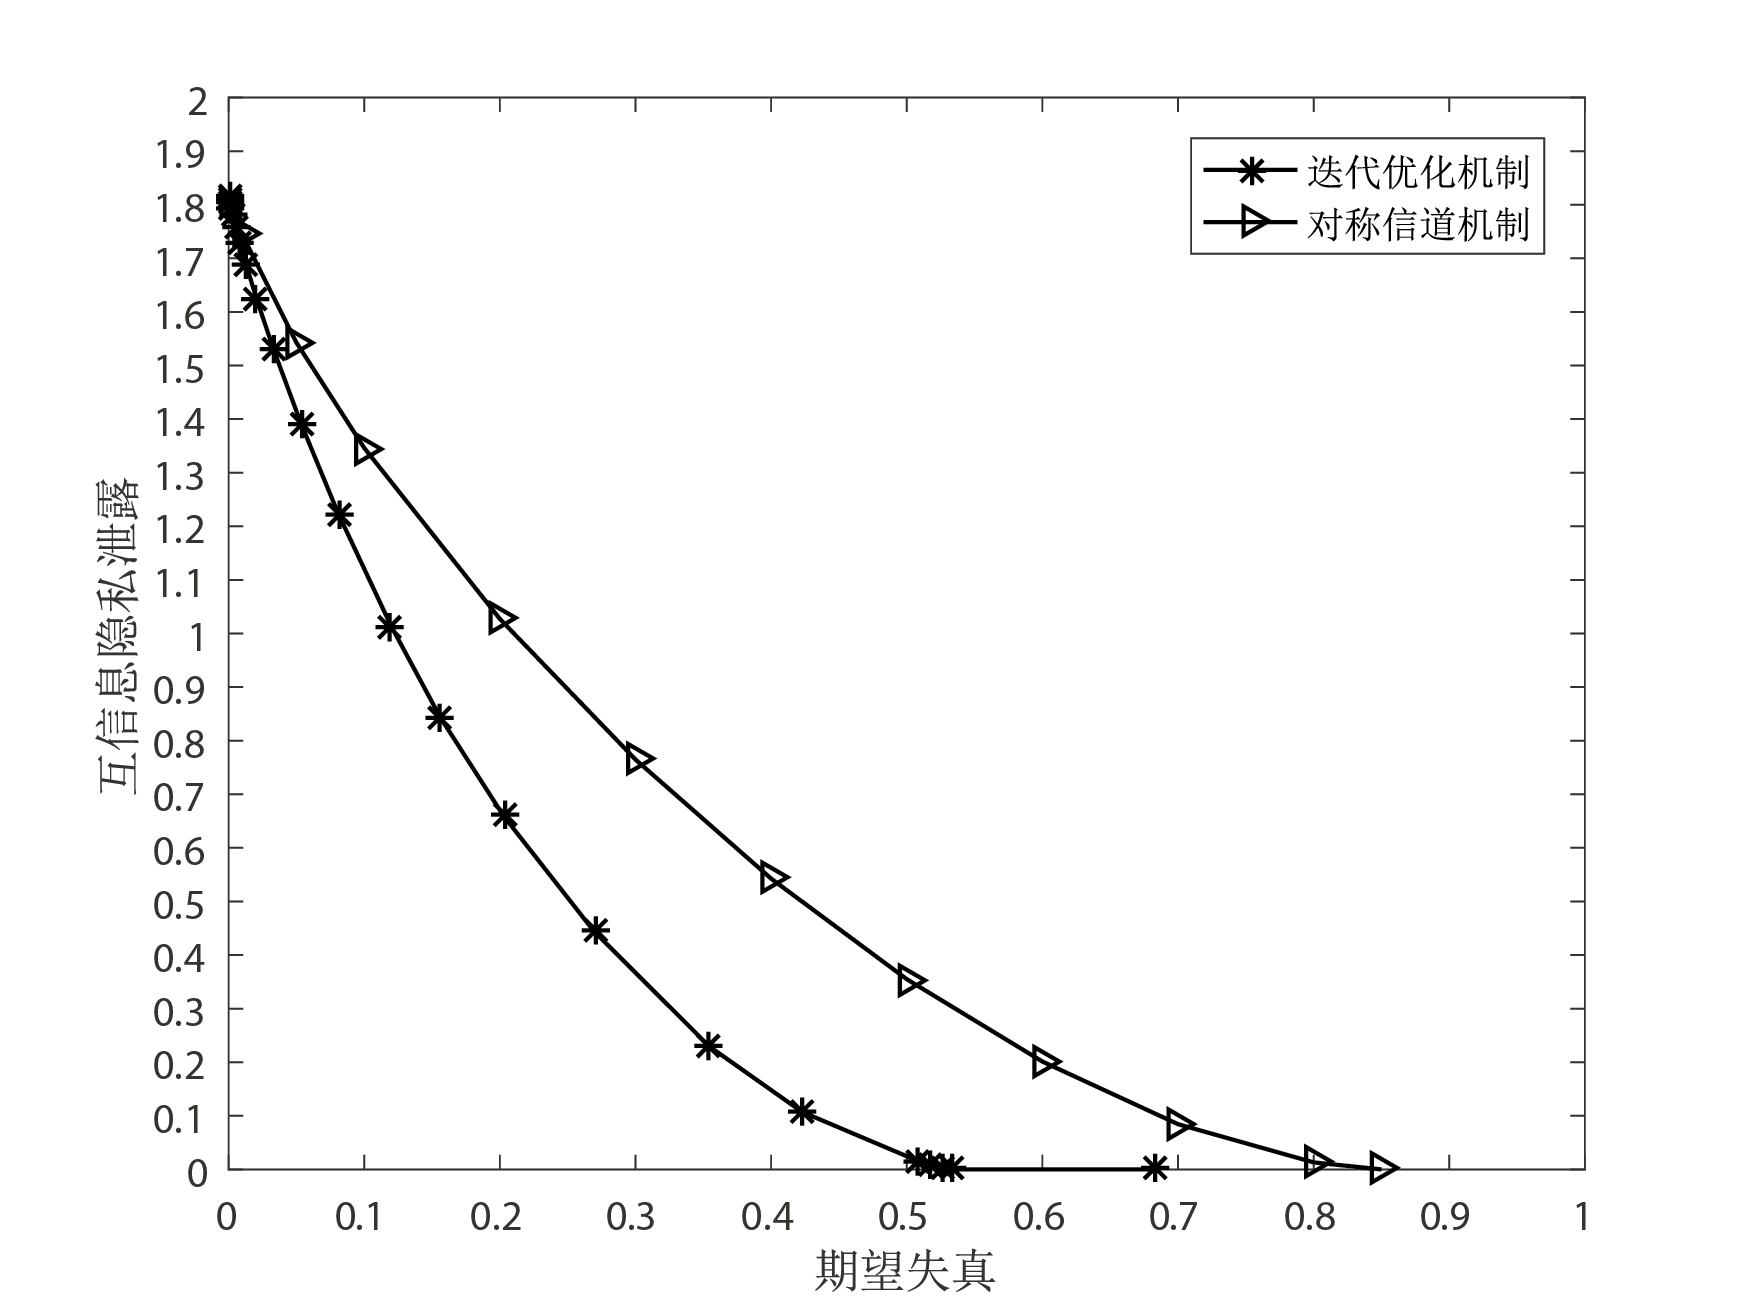
\includegraphics[width=3.5in]{chapter04/Figure6.png}
\caption{两种差分隐私信道机制的对比}
\label{Fig:chapter05-6}
\end{figure}

以下基于本文的隐私与效用度量方法给出实验结果与分析。首先,通过本章中迭代算法求解的隐私信道机制与对称的信道机制在互信息隐私和期望失真度量方面进行对比,比较隐私与数据效用性能。两种不同的信道条件概率分布之间,互信息隐私和期望失真的变化曲线如图\ref{Fig:chapter05-6}所示。图中曲线所示的结果分析,本章中通过优化模型迭代算法求解的隐私机制在同等失真度条件下比对称信道机制表现出更小的互信息隐私泄露。为详细的、定量的表述两种不同隐私机制之间的比较。表\ref{tab:chapter05-1}给出了限失真的互信息隐私泄露量对比数据,表达出同等失真度条件下,迭代优化机制具有相对较小的隐私泄露量。与之对应的,表\ref{tab:chapter05-2}的数据表现出同等隐私泄露容忍度条件下,迭代优化机制拥有相对较小的失真度。结合图\ref{Fig:chapter05-6}及表\ref{tab:chapter05-1}得知,在满足数据质量损失约束前提下,所求解的迭代优化机制比对称信道机制有较好的隐私效果。


\begin{table}
\setstretch{1.1}
\centering
\caption{限失真的互信息隐私泄露量对比}
\label{tab:chapter05-1}
\begin{tabular}{ccc}
  \hline
    机制对比 & 互信息泄露量 & 期望失真\\
  \hline
  对称信道机制 & \tabincell{c}{(0.3397, 0.4963, 0.6379, 0.8387) \\ (1.0185, 1.1587, 1.2761, 1.4166)\\(1.5428, 1.6205, 1.6813, 1.7261)}
   & \multirow{3}{*}{\tabincell{c}{(0.509, 0.423, 0.355, 0.270)\\(0.203, 0.156, 0.120, 0.081) \\ (0.050, 0.033, 0.021, 0.013)}}  \\ 	\cline{1-2}
    迭代优化机制 &  \tabincell{c}{(0.0154, 0.1073, 0.2293, 0.4437) \\ (0.6593, 0.8440, 1.0143, 1.2242)\\(1.3923, 1.5290, 1.6237, 1.6880)}
  &   \\
  \cline{1-3}
\end{tabular}
\end{table}

% \begin{table}[!h]
\begin{table}
\setstretch{1.1}
\centering
\caption{相同互信息隐私泄露的期望失真度对比}
\label{tab:chapter05-2}
\begin{tabular}{ccc}
  \hline
    机制对比 & 期望失真 & 互信息泄露量\\
  \hline
  对称信道机制 & \tabincell{c}{(0.780, 0.675, 0.580) \\ (0.450, 0.345, 0.270)\\(0.205, 0.050, 0.020)}
   & \multirow{3}{*}{\tabincell{c}{(0.02, 0.11, 0.23) \\ (0.44, 0.66, 0.84) \\ (1.01, 1.54, 1.69)}}  \\ 	\cline{1-2}
    迭代优化机制 &  \tabincell{c}{(0.509, 0.423, 0.355) \\ (0.270, 0.203, 0.156)\\(0.120, 0.033, 0.013)}
  &   \\
  \cline{1-3}
\end{tabular}
\end{table}

\begin{figure}[htbp]
\centering
\begin{minipage}[t]{0.48\textwidth}
\centering
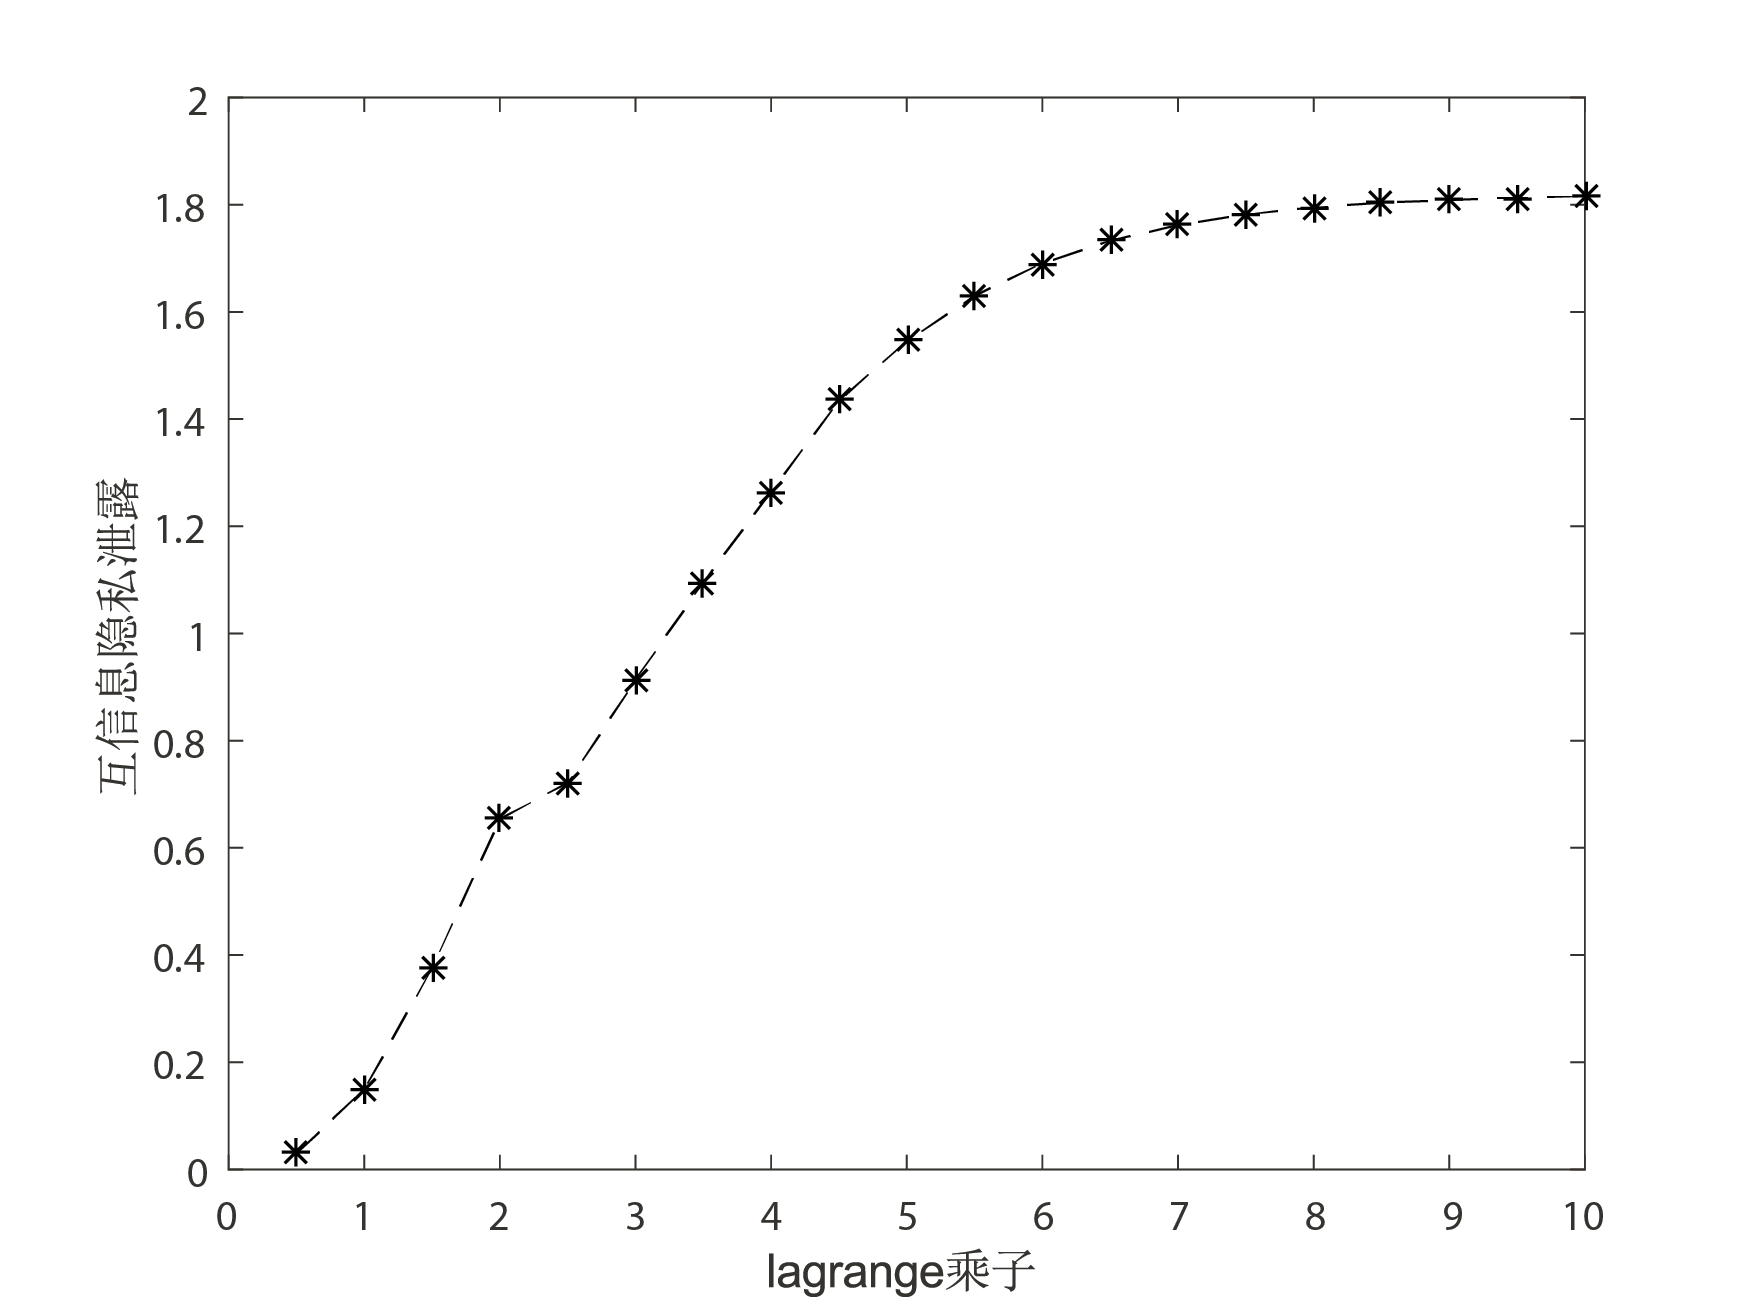
\includegraphics[width=8cm]{chapter04/Figure7.png}
\caption{拉格朗日乘子与互信息隐私泄露}
\label{Fig:chapter05-7}
\end{minipage}
\begin{minipage}[t]{0.48\textwidth}
\centering
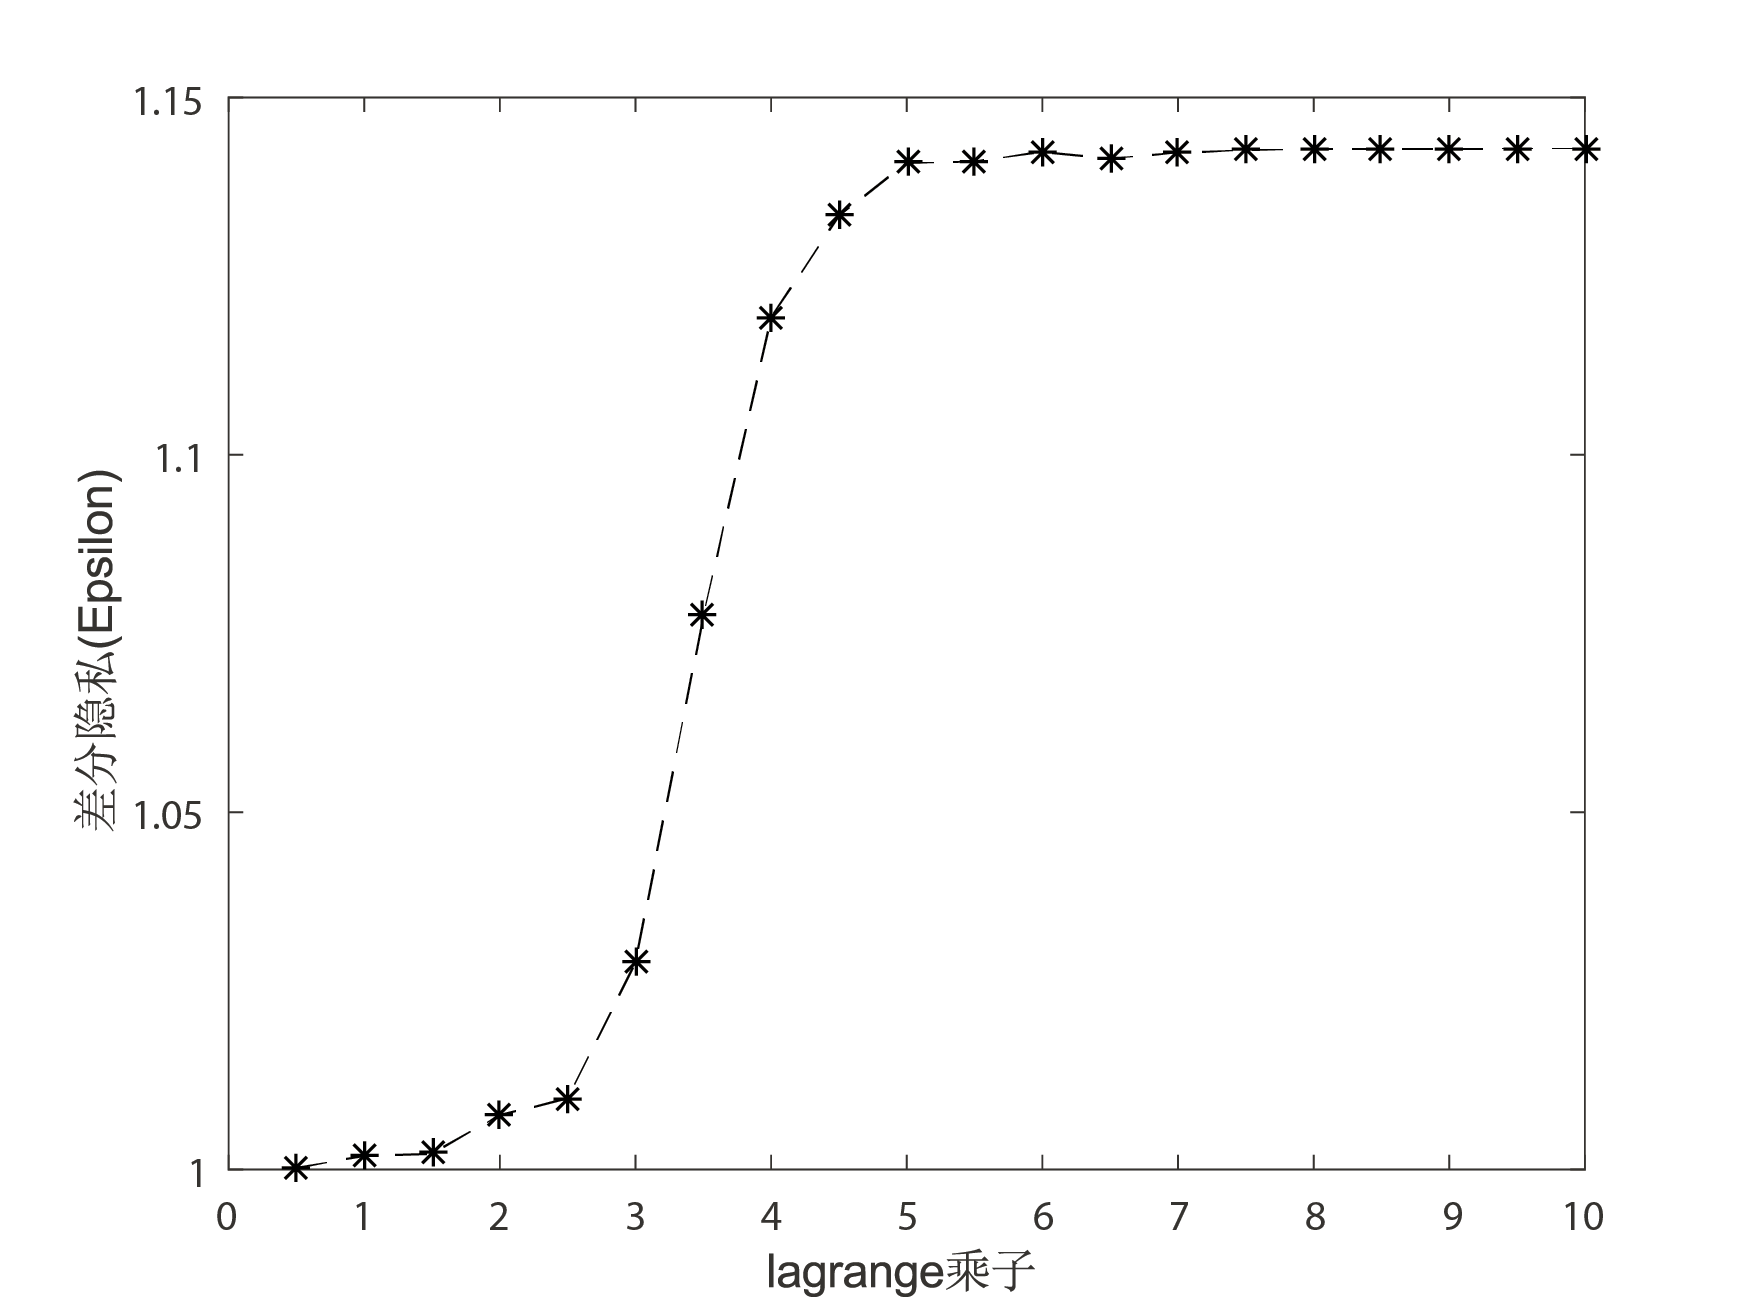
\includegraphics[width=8cm]{chapter04/Figure8.png}
\caption{具有辅助背景知识的$\lambda$与隐私参数}
\label{Fig:chapter05-8}
\end{minipage}
\end{figure}

为研究优化模型$2$的迭代算法中参数对隐私机制条件概率分布的影响,选取$\lambda \in [0.5,10]$,$T=0.01$分析$\lambda$和互信息隐私泄露量、预算参数之间的变化关系。首先,图\ref{Fig:chapter05-7}中展示了$\lambda$和互信息隐私泄露量的变化曲线,结果表明随着$\lambda$的增加,隐私机制的保护强度减弱,互信息隐私泄露量增大。除此之外,曲线的斜率表明了随$\lambda$变大隐私泄露量的增长率下降。当$\lambda \geq 5$时,隐私泄露的变化逐渐呈现平稳的发展趋势。相对应的,隐私预算参数的变化曲线图\ref{Fig:chapter05-8}(图中以$\ln$为单位),结果表明$\lambda$的增加带动了隐私参数的增长,刻画了隐私保护强度的减弱。当$\lambda \geq 5$时,图\ref{Fig:chapter05-8}所表明的结果与图\ref{Fig:chapter05-7}中的结果具有一致性。

更多地,阐述算法中参数$\lambda$,$T$和互信息隐私泄露、期望失真度的关系。实验中设置$\lambda \in \{0.5,1.0,1.5,2.0,2.5\}$、$T\in \{10^{-4},10^{-5},10^{-6},10^{-7},10^{-8}\}$,并组合考虑了不同的$\lambda$和$T$组合。以下给出实验结果的描述。首先,互信息隐私方面,固定$T$ 的取值改变$\lambda$的实验结果如图\ref{Fig:chapter05-9}所示。图中的结果表明,随$\lambda$增加互信息隐私泄露量变大。同时可以看出,选定$\lambda$,$T$的步长以$10$的倍数增长时,互信息隐私泄露量变化较微弱。其次,期望失真的数据质量损失方面,$\lambda$,$T$和期望失真的变化关系如图\ref{Fig:chapter05-10} 所示。图中的结果表明选定$T$时,$\lambda$的变大使得失真损失增加。然而,选定$\lambda$具体取值时,以步长为$10$的数量级增长的$T$并没有引起期望失真的明显变化。基于此说明,在通过算法求解最优信道条件概率分布,设计隐私保护机制阶段,考虑隐私与数据质量需求恰当的选择算法参数$\lambda$和$T$,获得理想的隐私保护效果。
\begin{figure}[htbp]
\centering
\begin{minipage}[t]{0.48\textwidth}
\centering
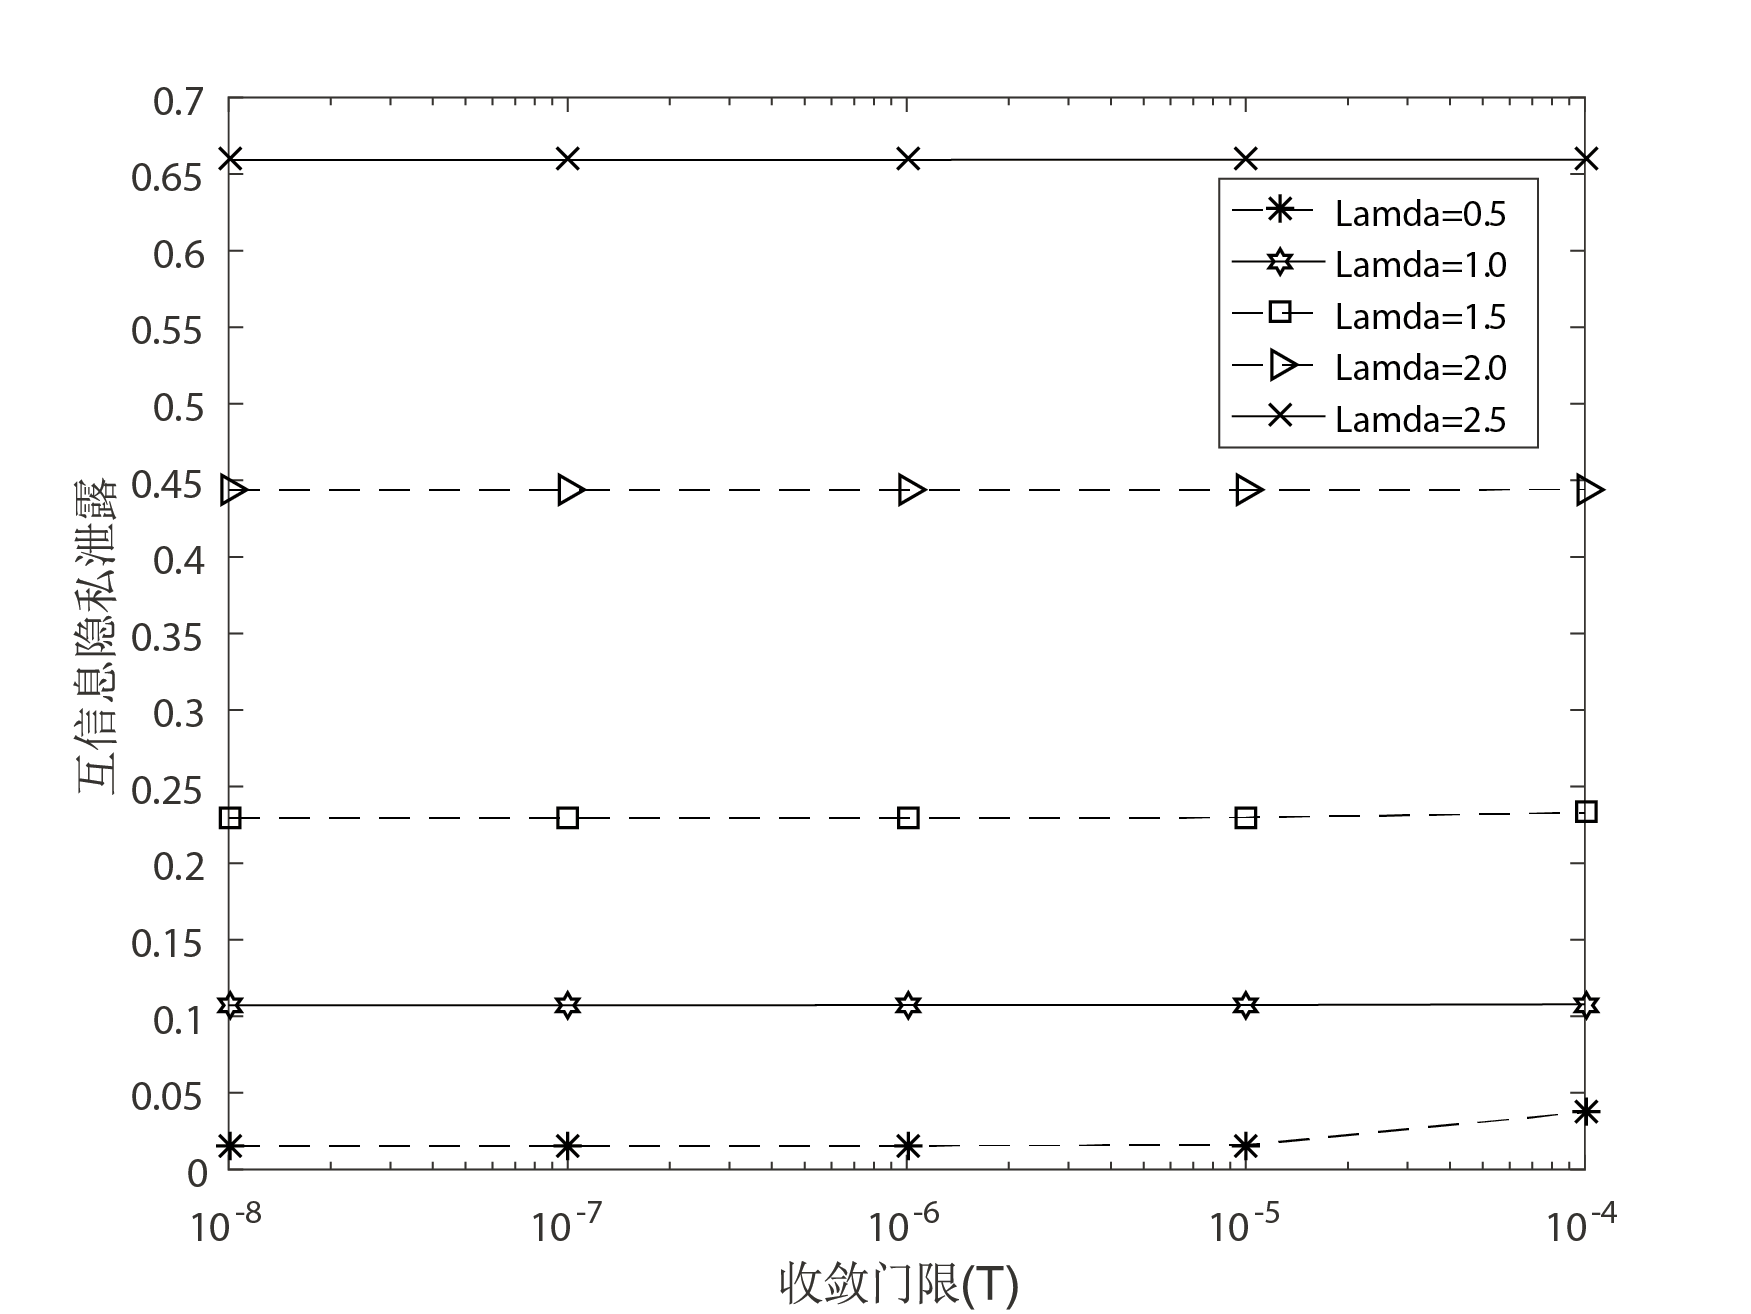
\includegraphics[width=8cm]{chapter04/Figure9.png}
\caption{收敛门限与互信息隐私泄露量}
\label{Fig:chapter05-9}
\end{minipage}
\begin{minipage}[t]{0.48\textwidth}
\centering
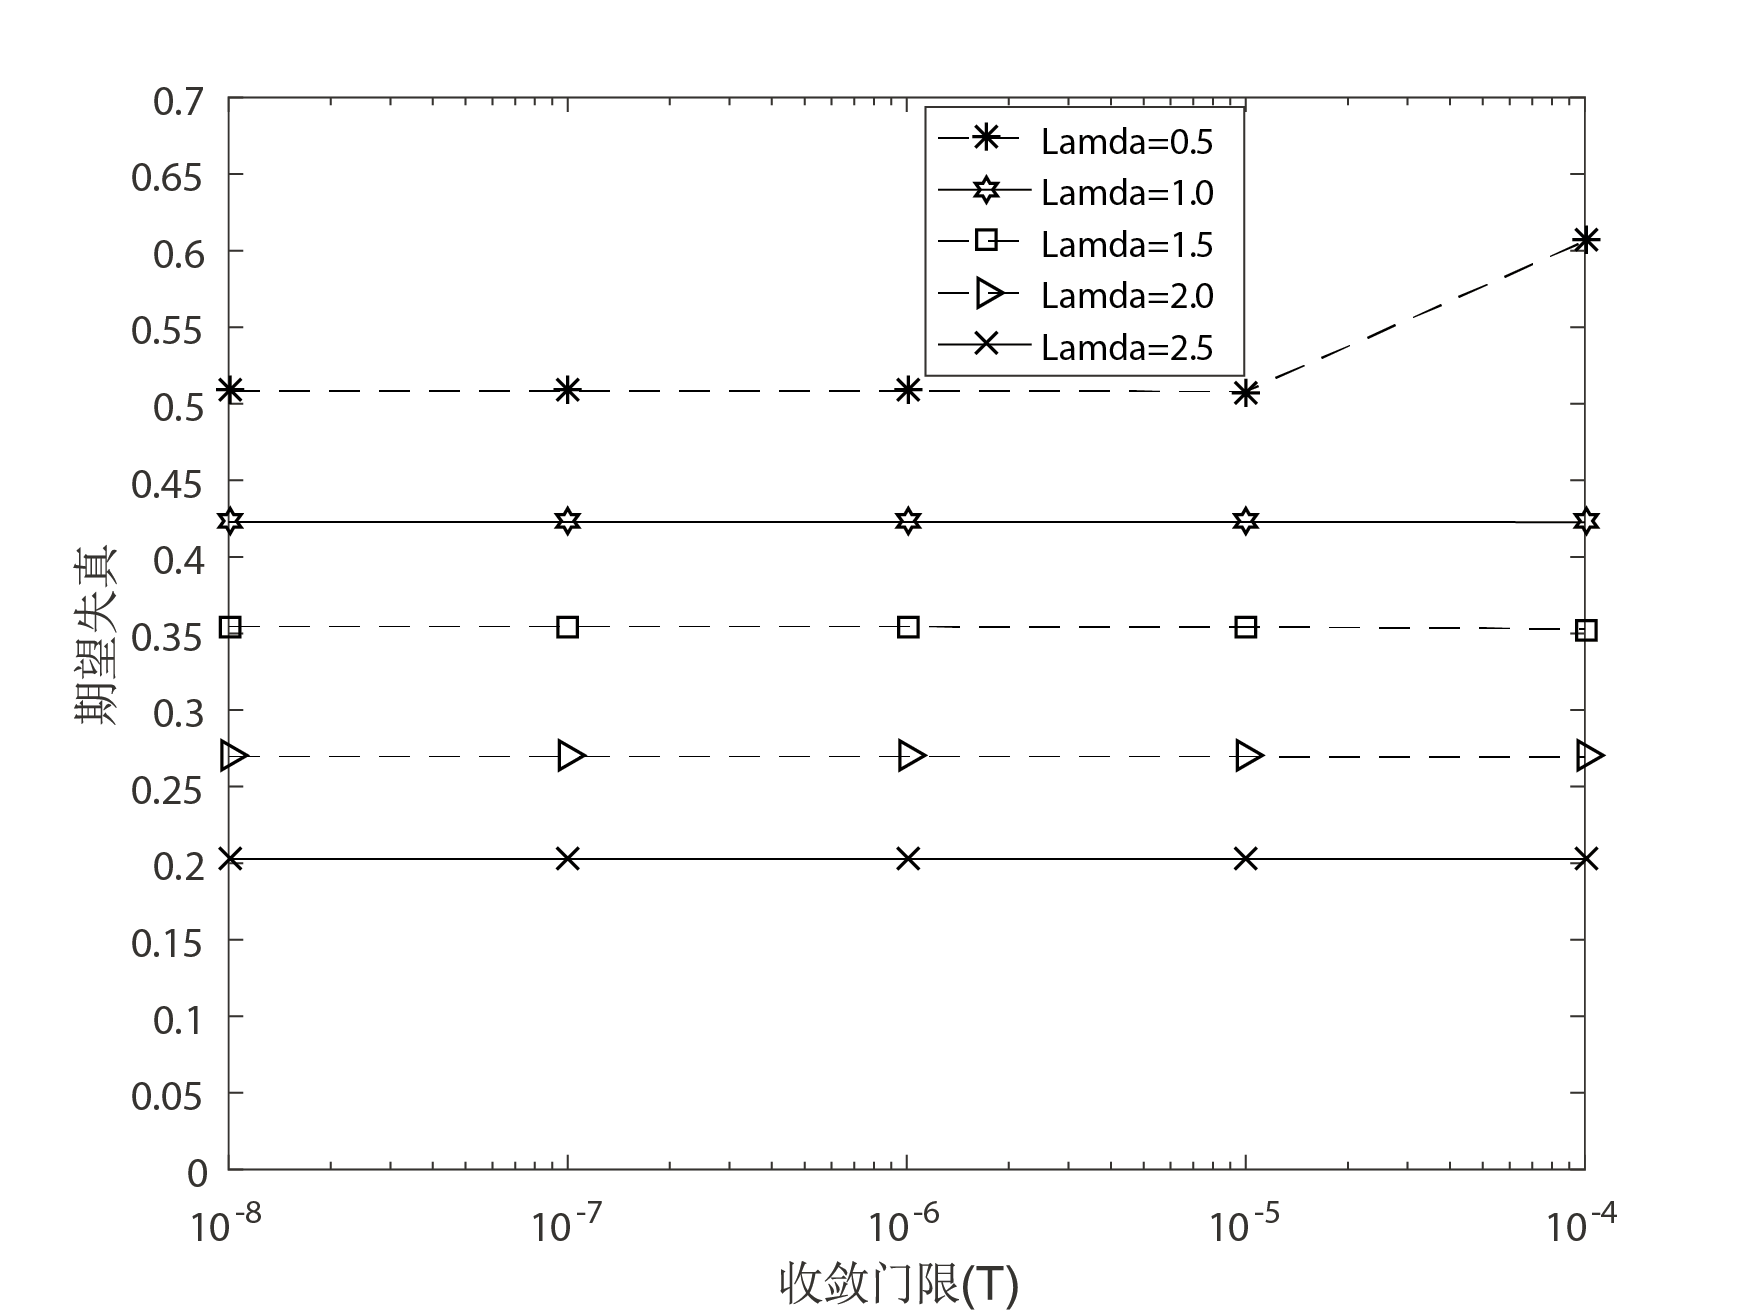
\includegraphics[width=8cm]{chapter04/Figure10.png}
\caption{收敛门限与期望失真度}
\label{Fig:chapter05-10}
\end{minipage}
\end{figure}



本节针对差分隐私数据发布应用中隐私攻击者有或无辅助背景知识的优化模型$1$和$2$,分别采用真实的数据集进行了实验,给出最优化模型迭代计算的差分隐私信道机制在互信息隐私泄露、期望失真方面的分析。在模型$2$求解的隐私机制中,基于隐私与数据可用性的信息论度量对比了对称信道机制。数据结果表明本章中考虑背景知识条件下的迭代优化机制在相同失真下具有比较小的隐私泄露,在相同隐私泄露条件下,所提出的方法具有较高的数据效用。

\section{本章小结}\label{chapter04-conclusion}
本章针对差分隐私数据发布中的隐私保护问题,借鉴Shannon信息论基本通信模型,在隐私与数据效用的度量基础上,利用率失真理论构建了隐私与失真的最优化模型,研究了满足数据质量损失约束条件的互信息隐私最优化机制问题,给出差分隐私数据发布的互信息隐私优化模型。随后,在数据发布的隐私通信模型中,考虑了隐私攻击者可能具有的关联辅助背景知识对互信息隐私泄露的影响,提出了基于联合事件的最小化互信息隐私泄露的优化模型。对于模型求解计算信道条件概率分布的问题,利用拉格朗日乘子法和凸问题的KKT最优性条件,给出解的参量表达式。在迭代算法计算方面,基于率失真函数求解的Blahut-Arimoto算法设计了最优化信道条件概率的迭代求解算法。最后,通过真实数据集上的实验结果,阐述了本章理论部分的研究成果,分析了所提出模型及算法的有效性及优势。

